% ---------- Titelblad Masterproef Faculteit Wetenschappen -----------
% Dit document is opgesteld voor compilatie met pdflatex.  Indien je
% wilt compileren met latex naar dvi/ps, dien je de figuren naar
% (e)ps-formaat om te zetten.
%                           -- december 2012
% -------------------------------------------------------------------
\RequirePackage{fix-cm}
\documentclass[12pt,a4paper,oneside]{book}

% --------------------- In te laden pakketten -----------------------
% Deze kan je eventueel toevoegen aan de pakketten die je al inlaadt
% als je dit titelblad integreert met de rest van thesis.
% -------------------------------------------------------------------
\usepackage[dutch]{babel}
\usepackage{graphicx,xcolor,textpos}
\usepackage[utf8]{inputenc}
\usepackage[T1]{fontenc}
\usepackage{helvet}
\usepackage{amsmath}
\usepackage{listings}
\usepackage{hyperref}
\usepackage[hypcap]{caption}
\usepackage{color}
\usepackage{longtable}
\usepackage{booktabs}
\usepackage{pgfplotstable}
\usepackage{needspace}
\usepackage[toc,page]{appendix}
\usepackage{ltablex}

% -------------------- Pagina-instellingen --------------------------
% Indien je deze wijzigt, zal het titelblad ook wijzigen.  Dit dien je
% dan manueel aan te passen.
% --------------------------------------------------------------------
\topmargin -10mm
\textwidth 160truemm
\textheight 240truemm
\oddsidemargin 0mm
\evensidemargin 0mm

% ------------------- textpos-instellingen ---------------------------
% Enkele andere instellingen voor het voorblad.
% --------------------------------------------------------------------
\definecolor{green}{RGB}{172,196,0}
\definecolor{bluetitle}{RGB}{29,141,176}
\definecolor{blueaff}{RGB}{0,0,128}
\definecolor{blueline}{RGB}{82,189,236}
\definecolor{dkgreen}{rgb}{0,0.6,0}
\definecolor{gray}{rgb}{0.5,0.5,0.5}
\definecolor{mauve}{rgb}{0.58,0,0.82}
\setlength{\TPHorizModule}{1mm}
\setlength{\TPVertModule}{1mm}

% Eigen instellingen
%\setdefaultlanguage{dutch}
\newcommand{\powerTable}[3]{
    \Needspace{15\baselineskip}
    \pgfplotstabletypeset[
        string type,
        col sep = comma,
        skip rows between index={0}{#2},
        skip rows between index={#3}{1000000000},
        begin table=\begin{longtable},
        end table=\end{longtable},
        % packo id,N,Packomania Radius,,id,circlecount,Radius,time (ns),overlap (square units),nancount,Time,,Difference,% Increase
        columns={{N},{ratio},{Radius},{Difference},{Increase},{Time}},
        every head row/.style={before row=\caption[]{#1}\\\toprule, after row=\midrule\endhead},
        every last row/.style={after row=\bottomrule},
        every first row/.style={before row=\captionsetup{labelformat=empty}\caption[#1]{}\\[-23pt]},
        column type={l}, %default
        columns/{N}/.style={column type={c}},
        columns/{ratio}/.style={column name={Beste radius}},
        columns/{Radius}/.style={column name={Radius}},
        columns/{Difference}/.style={column name={Vergroting}},
        columns/{Increase}/.style={column type={c}, column name={Vergroting (\%)}},
        columns/{Time}/.style={column name={Tijd}},
    ]{csv/Power Packomania Problems Comparison.csv}
}





\newcommand{\equalTable}[3]{
    \Needspace{15\baselineskip}
    \pgfplotstabletypeset[
        string type,
        col sep = comma,
        skip rows between index={0}{#2},
        skip rows between index={#3}{1000000000},
        begin table=\begin{longtable},
        end table=\end{longtable},
        % N,radius,distance,ratio,density,contacts,loose,boundary,symmetry group,reference,,id,circlecount,Radius,time (ns),overlap (square units),nancount,Time,,Difference,Increase
        columns={{N},{ratio},{Radius},{Difference},{Increase},{Time}},
        every head row/.style={before row=\caption[]{#1}\\\toprule, after row=\midrule\endhead},
        every last row/.style={after row=\bottomrule},
        every first row/.style={before row=\captionsetup{labelformat=empty}\caption[#1]{}\\[-23pt]},
        column type={l}, %default
        columns/{N}/.style={column type={c}},
        columns/{ratio}/.style={column name={Beste radius}},
        columns/{Radius}/.style={column name={Radius}},
        columns/{Difference}/.style={column name={Vergroting}},
        columns/{Increase}/.style={column type={c}, column name={Vergroting (\%)}},
        columns/{Time}/.style={column name={Tijd}},
    ]{csv/Equal size Packomania problems comparison.csv}
}





\newcommand{\benchmarkTable}[3]{
    \Needspace{15\baselineskip}
    \pgfplotstabletypeset[
        string type,
        col sep = comma,
        skip rows between index={0}{#2},
        skip rows between index={#3}{1000000000},
        begin table=\begin{longtable},
        end table=\end{longtable},
        % instance,N,radius,ratio,density,,id,circlecount,Radius,time (ns),overlap (square units),nancount,Time,,Difference,Increase
        columns={{instance},{N},{ratio},{Radius},{Difference},{Increase},{Time}},
        every head row/.style={before row=\caption[]{#1}\\\toprule, after row=\midrule\endhead},
        every last row/.style={after row=\bottomrule},
        every first row/.style={before row=\captionsetup{labelformat=empty}\caption[#1]{}\\[-23pt]},
        column type={l}, %default
        columns/{instance}/.style={column name={Instantie}},
        columns/{N}/.style={column type={c}},
        columns/{ratio}/.style={column name={Beste radius}},
        columns/{Radius}/.style={column name={Radius}},
        columns/{Difference}/.style={column name={Vergroting}},
        columns/{Increase}/.style={column type={c}, column name={Vergroting (\%)}},
        columns/{Time}/.style={column name={Tijd}},
    ]{csv/IN NR Packomania problems comparison.csv}
}

\graphicspath{{images/}}
\renewcommand{\contentsname}{Inhoud}
\renewcommand{\listfigurename}{Lijst van figuren}
\renewcommand{\listtablename}{Lijst van tabellen}
\renewcommand{\chaptername}{Hoofdstuk}
\renewcommand{\chapterautorefname}{hoofdstuk}
\renewcommand{\sectionautorefname}{sectie}
\renewcommand{\subsectionautorefname}{sectie}
\renewcommand{\figureautorefname}{figuur}
\renewcommand{\tableautorefname}{tabel}
\newcommand{\lstnumberautorefname}{lijn}
\renewcommand{\appendixautorefname}{bijlage}

\lstset{frame=tb,
  language=Java,
  aboveskip=3mm,
  belowskip=3mm,
  showstringspaces=false,
  columns=flexible,
  basicstyle={\small\ttfamily},
  numbers=left,
  numberstyle=\tiny\color{gray},
  keywordstyle=\color{blue},
  commentstyle=\color{dkgreen},
  stringstyle=\color{mauve},
  breaklines=true,
  breakatwhitespace=true,
  tabsize=4,
  escapechar=|
}

% begin appendix autoref patch [\autoref subsections in appendix](http://tex.stackexchange.com/questions/149807/autoref-subsections-in-appendix)
\usepackage{etoolbox}
\makeatletter
\patchcmd{\hyper@makecurrent}{%
    \ifx\Hy@param\Hy@chapterstring
        \let\Hy@param\Hy@chapapp
    \fi
}{%
    \iftoggle{inappendix}{%true-branch
        % list the names of all sectioning counters here
        \@checkappendixparam{chapter}%
        \@checkappendixparam{section}%
        \@checkappendixparam{subsection}%
        \@checkappendixparam{subsubsection}%
        \@checkappendixparam{paragraph}%
        \@checkappendixparam{subparagraph}%
    }{}%
}{}{\errmessage{failed to patch}}

\newcommand*{\@checkappendixparam}[1]{%
    \def\@checkappendixparamtmp{#1}%
    \ifx\Hy@param\@checkappendixparamtmp
        \let\Hy@param\Hy@appendixstring
    \fi
}
\makeatletter

\newtoggle{inappendix}
\togglefalse{inappendix}

\apptocmd{\appendix}{\toggletrue{inappendix}}{}{\errmessage{failed to patch}}
\apptocmd{\subappendices}{\toggletrue{inappendix}}{}{\errmessage{failed to patch}}
% end appendix autoref patch

\begin{document}

% ---------------------- Voorblad ------------------------------------
% Vergeet niet de tekst aan te passen:
% - Titel en, indien van toepassing, ondertitel
%          voor eventuele formules in de titel of ondertitel
%          gebruik je  \form{$...$}
% - Je naam
% - Je (co)promotor, begeleider (indien van toepassing)
% - Je opleiding
% - Het academiejaar
% --------------------------------------------------------------------
\thispagestyle{empty}
\newcommand{\form}[1]{\scalebox{1.087}{\boldmath{#1}}}
\sffamily
%
\begin{textblock}{191}(-24,-11)
\colorbox{green}{\hspace{123mm}\ \parbox[c][18truemm]{68mm}{\textcolor{white}{FACULTEIT WETENSCHAPPEN}}}
\end{textblock}
%
\begin{textblock}{70}(-18,-19)
\textblockcolour{}
\includegraphics*[height=19.8truemm]{LogoKULeuven.png}
\end{textblock}
%
\begin{textblock}{79}(50,50)
\centerline{\includegraphics*[height=10.0truecm]{voorbladpacking_75.png}}
%De achtergrond kan wit blijven of je kan een afbeelding invoegen (maximum hoogte 10 cm, breedte variabel, denk aan auteursrechten\ldots). GEEN logo's (je kan binnenin de masterproef logo's gebruiken, maar niet op de voor- of achterpagina).
\end{textblock}
%
\begin{textblock}{160}(-6,63)
\textblockcolour{}
\vspace{-\parskip}
\flushleft
\fontsize{40}{42}\selectfont \textcolor{bluetitle}{Een nieuwe constructieve heuristiek voor het \textit{circle-packing} probleem}\\[1.5mm]
\fontsize{20}{22}\selectfont Gebaseerd op een \textit{best-fit} methodiek
\end{textblock}
%
\begin{textblock}{160}(8,153)
\textblockcolour{}
\vspace{-\parskip}
\flushright
\fontsize{14}{16}\selectfont \textbf{Pablo BOLLANSÉE}
\end{textblock}
%
\begin{textblock}{70}(-6,191)
\textblockcolour{}
\vspace{-\parskip}
\flushleft
Promotor:\\ Prof. dr. Patrick De Causmaecker \\[-2pt]
\textcolor{blueaff}{KU Leuven, Departement Computerwetenschappen, CODeS@KULAK}\\[5pt]
%Co-promotor: \textsl{(facultatief)}\\[-2pt]
%\textcolor{blueaff}{Affiliatie \textsl{(facultatief)}}\\[5pt]
%Begeleider: \textsl{(facultatief)}\\[-2pt]
%\textcolor{blueaff}{Affiliatie \textsl{(facultatief)}}\\
\end{textblock}
%
\begin{textblock}{160}(8,191)
\textblockcolour{}
\vspace{-\parskip}
\flushright
Proefschrift ingediend tot het\\[4.5pt]
behalen van de graad van\\[4.5pt]
Master of Science in de\\[4.5pt]
toegepaste informatica\\
\end{textblock}
%
\begin{textblock}{160}(8,232)
\textblockcolour{}
\vspace{-\parskip}
\flushright
Academiejaar 2015-2016
\end{textblock}
%
\begin{textblock}{191}(-24,248)
{\color{blueline}\rule{550pt}{5.5pt}}
\end{textblock}
%
\vfill

\newpage
\thispagestyle{empty}
\begin{textblock}{160}(0,185)
© Copyright by KU Leuven

Zonder voorafgaande schriftelijke toestemming van zowel de promotor(en) als de auteur(s) is overnemen, kopiëren, gebruiken of realiseren van deze uitgave of gedeelten ervan verboden. Voor aanvragen tot of informatie i.v.m. het overnemen en/of gebruik en/of realisatie van gedeelten uit deze publicatie, wendt u tot de KU Leuven, Faculteit Wetenschappen, Geel Huis, Kasteelpark Arenberg 11 bus 2100, 3001 Leuven (Heverlee), Telefoon +32 16 32 14 01.

Voorafgaande schriftelijke toestemming van de promotor(en) is eveneens vereist voor het aanwenden van de in dit afstudeerwerk beschreven (originele) methoden, producten, schakelingen en programma’s voor industrieel of commercieel nut en voor de inzending van deze publicatie ter deelname aan wetenschappelijke prijzen of wedstrijden.
\end{textblock}

\newpage

% Als je het titelblad wil integreren met de rest van je thesis,
% kan je hieronder verder.
% ----------------------- Eerste pagina's -------------------------
% Hier kan je inhoudsopgave, voorwoord en dergelijke kwijt.
% -----------------------------------------------------------------
\rmfamily
\setcounter{page}{0}
\pagenumbering{roman}

\newpage

\chapter*{Voorwoord}
\addcontentsline{toc}{chapter}{Voorwoord}

Het \textit{circle-packing} probleem bestaat er uit om een aantal cirkels, met gekende radii, in een zo klein mogelijke \textit{container} te plaatsen.
De vorm van deze \textit{container} kan verschillen, meestal is het een driehoek, rechthoek of cirkel.
In deze thesis stel ik een nieuwe heuristiek voor het plaatsen van cirkels in een cirkel voor, gebaseerd op het \textit{best-fit}-principe.
Het is een constructieve heuristiek waarin stapsgewijs telkens de best-passende cirkel geplaatst zal worden.
Alle broncode is beschikbaar op GitHub \cite{circle-packing-github}

Hoewel dit probleem wiskunig relatief eenvoudig voor te stellen is, is het uitwerken van een computioneel exacte oplossing wél een uitdaging.
Bestaande implementaties zijn niet tijds-geoptimaliseerd, en vragen dus veel berekeningstijd. 
In deze thesis stek ik een nieuwe heuristiek voor die het mogelijk maakt zéér snel oplossingen te genereren.

Dit werk werd gedaan als masterproef voor de \textit{Master of Science in de toegepaste informatica} te KU Leuven onder de CODeS onderzoeksgroep.
Het hield 18 studiepunten in van deze éénjarige master.

Ik wil hierbij Patrick De Causmaeker bedanken voor alle hulp en ondersteuning bij het ontwerpen van deze heuristiek en verwezenlijken van dit werk.
Ook wil ik Jim Bollansée, Marie Julia Bollansée en Pieter Van de Walle bedanken voor hun hulp bij het schrijven van deze tekst.

%  In het voorwoord wordt de algemene doelstelling van het werk samengevat
%  in enkele regels en worden personen, diensten of firma’s bedankt voor hun
%  medewerking bij het tot stand komen van het werk.
%  De naam van firma’s en personen uit deze firma’s mogen slechts worden vermeld
%  mits hun uitdrukkelijke toelating én na overleg met de supervisor(en)! Steeds
%  wordt de supervisor(en) vermeld, de verantwoordelijke en eventueel de personen
%  die rechtstreeks geholpen hebben bv. door het ter beschikking stelling van
%  meetresultaten, faciliteiten. Ook de instantie die eventueel een doctoraatsbeurs
%  heeft toegekend wordt bedankt (bv. FWO, IWT, . . . ).

\newpage

\chapter*{Abstract}
\addcontentsline{toc}{chapter}{Abstract}

%  In een beknopte tekst van maximum 2 pagina’s worden de belangrijkste
%  doelstellingen en besluiten geformuleerd, zowel in het Nederlands als in het
%  Engels. Zulke samenvattingen kunnen worden gebruikt in wetenschappelijke
%  verslagen van het departement of de faculteit. Het Engels moet vlekkeloos zijn.

Het \textit{circle-packing} probleem bestaat er uit om een aantal cirkels, met gekende radii, in een zo klein mogelijke \textit{container} te plaatsen.
De vorm van deze \textit{container} kan verschillen, meestal is het een driehoek, rechthoek of cirkel.
In deze thesis stel ik een nieuwe \textit{best-fit} gebaseerde heuristiek voor het plaatsen van cirkels in een cirkel voor.
Het is een constructieve heuristiek waarin stapsgewijs telkens de \textit{best-passende} cirkel geplaatst zal worden.

Wiskundig is dit een relatief eenvoudig probleem om voor te stellen, maar computationeel is het zeer zwaar om exact op te lossen.
Bestaande pogingen om dit probleem op te lossen vragen zeer veel tijd om het te berekenen.
In deze thesis stel ik een nieuwe heuristiek voor die het mogelijk maakt zéér snel oplossingen te genereren.

Oplossingen gegenereerd door het algoritme uit deze thesis hebben een omschreven cirkel die gemiddeld minder dan 6\% groter is in vergelijking met de best gekende oplossingen.
Dit is een zeer aanvaardbare uitbreiding van de omschreven cirkel, toch als je in rekening brengt dat deze oplossingen veel sneller bekomen zijn.
Bestaande pogingen vragen uren en soms dagen tijd om slechts tientallen cirkels te plaatsen.
De heuristiek voorgesteld in deze thesis lost het probleen op in slechts enkele milliseconden.

Daarbovenop maakt deze heuristiek het mogelijk om nieuwe problemen op te lossen.
Zo zouden problemen met duizenden cirkels met voorgaande methoden onrealistisch veel tijd vragen, tientallen cirkels vragen al uren of dagen tijd.
Dit soort problemen kunnen wel opgelost worden met deze nieuwe heuristiek.

\newpage

\chapter*{Abstract (English)}
\addcontentsline{toc}{chapter}{Abstract (English)}

The \textit{circle-packing} problem consists of packing a number of circles, with given radii, in a container that is as small as possible.
The shape of this container can differ, but most often triangular, rectangular or circular.
In this thesis I propose a new \textit{best-fit} based heuristic to solve the problem of packing circles in a circle.
It's a new constructive heuristic that builds a solution step-by-step by iteratively placing the circle that \textit{fits best}.

Mathematically this is a relatively simple problem to model, but computationally it is very complex to solve.
Existing methods to solve this problem are very time consuming.
In this thesis I propose a new heuristic that can solve the problem in just a few milliseconds.

Solutions generated by the algorithm proposed in this thesis will result in a slight increase of radius of the circumscribed circle.
Compared to the best-known solutions this method results in a radius that is on average less then 6\% larger.
This is a very acceptable increase when considering that the results are computed much faster.
Existing methods require hours or days to compute a solution for just tens of circles.
The heuristic in this thesis will give a solution in just milliseconds for the same problems.

On top of that this new heuristic allows us to solve new problems. 
Problems with thousands of circles would take an unrealistic amount of time for older algorithms.
However for this new heuristic these problems aren't out of scope.

\newpage

\tableofcontents
\listoffigures
\addcontentsline{toc}{chapter}{Lijst van figuren}
\listoftables
\addcontentsline{toc}{chapter}{Lijst van tabellen}

\newpage

% ----------------------- Eigenlijke thesis -----------------------
% Vanaf de inleiding/het eerste hoofdstuk.
% -----------------------------------------------------------------
\setcounter{page}{0}
\pagenumbering{arabic}

\chapter{Inleiding}

In deze thesis stel ik een nieuwe heuristiek voor, gebaseerd op het \textit{best-fit}-principe, als oplossing voor het \textit{circle-packing} probleem.
De heuristiek is specifiek ontworpen voor het sub-probleem van het plaatsen van cirkels in een cirkel.
Het \textit{circle-packing} probleem bestaat uit het plaatsen van $n$ cirkels in een zo klein mogelijke cirkelvormige \textit{container}.
Het is de bedoeling om voor de gegeven cirkels de coordinaten van de middelpunten te vinden zodat de cirkels niet overlappen en de radius van de omschreven cirkel zo klein mogelijk is.

\textit{Circle-packing} is zowel theoretisch als praktisch een zeer interessant probleem.
Het kan gebruikt worden om verschillende \textit{real-world} problemen op te lossen, zoals het plaatsen van zendmasten, stockage van cilindrische voorwerpen, en het combineren van verschillende kabels. 
% //TODO voeg referenties toe voor deze gebruiken

Mathematisch is het probleem redelijk eenvoudig als een optimalisatieprobleem te omschrijven:

\begin{equation*}
\begin{aligned}
& \text{minimaliseer}
& & r \\
& \text{onderhevig aan}
& & x_i^2 + y_i^2 \leq (r-r_i)^2, 
& & &i = {1,...,n}\\
&&& (x_i - x_j)^2 + (y_i - y_j)^2 \geq (r_i + r_j)^2,
& & &i \neq j
\end{aligned}
\end{equation*}

Hierin is $r_i$ de radius, en $(x_i,y_i)$ de coördinaten van het centrum van cirkel $i$.
Hierbij wordt verondersteld dat de omcirkel het nulpunt als middelpunt heeft.
De eerste formule verzekert dat de cirkels in de omcirkel liggen, en de tweede dat ze elkaar niet overlappen.
Wanneer alle cirkels dezelfde grootte hebben, wordt meestal $r_i$ gelijk aan $1$ genomen.
Het \textit{circle-packing} probleem voor andere containers heeft gelijkaardige, relatief eenvoudige, wiskundige omschrijvingen.

Hoewel dit wiskundig eenvoudig te omschrijven is, blijft het toch een zeer moeilijk probleem om exact op te lossen.
Het is een NP-moeilijk probleem. Er is reeds veel onderzoek gebeurd naar het oplossen van het circle-packing probleem voor zowel cirkels van gelijke grootte, als voor cirkels van verschillende grootte.

In \cite{graham1996repeated} en \cite{lubachevsky1997curved} probeert men vaste patronen te vinden die een optimale \textit{packing} van cirkels met gelijke grootte geeft.
In \cite{graham1998dense} en \cite{wang2002improved} worden fysisch geïnspireerde simulaties gebruikt om \textit{packing} te bekomen.

In \cite{george1995packing} worden verschillende meta-heuristieken, waaronder een genetisch algoritme, uitgeprobeerd en vergeleken.
Zij ondervinden dat dit genetisch algoritme, alsook een quasi-random techniek, in vergelijking met de andere uitgeprobeerde meta-heuristieken, resultaten met de kleinste omschreven cirkel geven.
In \cite{hifi2004approximate} en \cite{hifi2004simulated} worden respectievelijk een genetisch en een \textit{simulated-annealing} algoritme voorgesteld.

Een recentere poging is het Monotonic Basin Hopping algoritme voorgesteld in \cite{grosso2010}.
Hierin beschrijven de onderzoekers dat er te veel lokale optima zijn voor een eenvoudige multi-start behandeling, en ze stellen als mogelijke oplossing een variant voor waarin ze op een slimme manier de beginpunten proberen te genereren.
Meer recent zijn \cite{jors2011} (2011), \cite{ye2013iterated} (2013) en \cite{zeng2016iterated} (2016).
Zij gebruiken de combinatorische eigenschappen van circle-packing in combinatie met een zoekmethode zoals \textit{tabu-search} en \textit{iterated local search} om een goede volgorde te vinden waarin de cirkels geplaatst kunnen worden.
In \cite{jors2011} plaatsen de onderzoekers zo één voor één elke cirkel en berekent een \textit{non-linear optimizer} hiervoor telkens een lokaal extremum voor de \textit{packing}.

Constructieve algoritmen voor het oplossen van \textit{circle-packings} zijn veel minder onderzocht en gedocumenteerd.
Een constructief algoritme is een algoritme dat, uitgaand van een zekere beginsituatie, stapsgewijs de oplossing uitbreidt tot deze volledig is.
Eén van de weinige constructieve methoden wordt beschreven in \cite{akeb2006basic}, waarin een alternatieve vorm van het \textit{circle-packing} probleem wordt opgelost. Bij deze variant ligt de grootte van de container vast, en er moeten zo veel mogelijk cirkels van gelijke grootte in deze container geplaatst worden.
In \cite{hifi2004approximate} wordt er een aanpassing gedaan op de klassieke \textit{bottom-left-first} heuristiek, voor het plaatsen van rechthoeken.
Deze heuristiek plaats rechthoeken zo ver mogelijk in de linker benedenhoek.
Dit is een zeer eenvoudige heuristiek die vaak goede resultaten geeft.
De onderzoekers hebben deze dan aangepast om cirkels in een rechthoek te plaatsen.

Hoewel veel van deze oplossingen zeer goede \textit{packings} maken, en regelmatig hun voorgangers verbeteren, vragen ze veel rekentijd en beperken ze zich tot een klein aantal cirkels.
Voor slechts tientallen cirkels kan de nodige rekentijd oplopen tot tientallen uren.
In deze thesis stel ik een nieuwe constructieve heuristiek voor om het \textit{circle-packing} probleem op te lossen.
Deze nieuwe heuristiek laat toe om \textit{packings} te maken in een fractie van de tijd die eerdere algoritmen daarvoor nodig hebben.
Ook is het mogelijk om veel grotere aantallen cirkels te plaatsen.
De omcirkel van \textit{packings} verkregen met deze nieuwe heuristiek is echter iets groter dan deze verkregen in eerder vernoemd onderzoek.
Deze uitbreiding van de omcirkel blijft echter beperkt en laat toe de \textit{packings} in slechts enkele ogenblikken te maken, waar andere oplossingen uren rekentijd vragen.

De heuristiek voorgesteld in deze thesis is een best-fit heuristiek gebaseerd op een oplossing voor het \textit{orthogonal stock-cutting problem} voorgesteld in \cite{burke2004new}.
In dit probleem worden balken geplaatst in een container met een vaste breedte, zodat de hoogte zo klein mogelijk blijft.
Deze heuristiek gebruikt het verschil tussen de breedte van een balk en een gat in de \textit{packing} als maatstaf voor de \textit{beste} positie.
Hun heuristiek kiest dus de volgende balk om te plaatsen uit een lijst, en plaatst deze op de \textit{beste} positie.
Op een gelijkaardige manier kiest mijn algoritme de volgende cirkel die best past in de huidige \textit{packing}.
Deze aanpak verschilt van het plaatsen van cirkels in een vooraf bepaalde volgorde zoals in \cite{grosso2010} en \cite{jors2011}.

In \autoref{chap:algoritme} bespreek ik hoe mijn heuristiek opgebouwd is.
Ik beschrijf de twee basisconcepten voor mijn \textit{best-fi}t heuristiek, de begrippen \textit{holes} en \textit{shell}, in detail.
Ik bespreek hoe deze concepten werken, en op welke manier gekozen wordt welke cirkel best past in de \textit{packing}.
Ik illustreer deze concepten verder door naar de implementatie te verwijzen.
In \autoref{chap:resultaten} worden de verkregen resultaten besproken.
Hier vergelijk ik de \textit{packings} met de best gekende resultaten zoals gerapporteerd op de Packomania website (\cite{packomania}).
Deze website verzamelt zo'n goed mogelijke oplossingen voor verschillende \textit{circle-packing} problemen, en bevat informatie over hun effectiviteit.
Ik vergelijk de omtrek van de verkregen omcirkel en de nodige tijd om de \textit{packing} te berekenen van mijn eigen heuristiek met de beste oplossingen op de Packomania website.
Ook toon ik resultaten voor \textit{packings} voor veel meer cirkels dan getoond op de Packomania website.
In \autoref{chap:bedenkingen} bespreek ik enkele bedenkingen die ik heb bij mijn onderzoek en de implementatie van de onderzochte heuristiek.
In \autoref{chap:verder-werk} bespreek ik mogelijke verbeteringen en ideeën voor verder onderzoek.
In \autoref{chap:handleiding-visualisaties} wordt kort verduidelijkt hoe de visualisaties, die doorheen deze thesis gebruikt worden, dienen geïnterpreteerd te worden.

In het eerstvolgende hoofdstuk (\autoref{chap:definities}) worden echter eerst enkele termen toegelicht die gebruikt worden in de verdere tekst, sommige uniek binnen  dit onderzoek.

% // TODO: Termen verduidelijken: meta-heuristiek, genetisch algoritme, quasi-random techniek, simulated-annealing, tabu-search, bottom-left-first heuristiek

\chapter{Definities en termen} \label{chap:definities}

\textbf{Cirkel}: In de literatuur rond \textit{circle-packing} en in deze thesis wordt het woord \textit{cirkel} of \textit{circle} gebruikt, maar eigenlijk zou het correcter zijn om \textit{schijf} te gebruiken. Dit geeft (onder andere) aan dat er een overlap tussen \textit{cirkel} is wanneer een cirkel volledig omringd is door een andere.
Voor twee cirkels met radii $r_a, r_b$ en coordinaten  $(x_a,y_a), (x_b,y_b)$ is er een overlap wanneer $r_a + r_b > \sqrt{(x_a-x_b)^2 + (y_a-y_b)^2}$. 

\textbf{Packing}: Vertaald als \textbf{plaatsing}. Een \textbf{packing} is een collectie cirkels met elk een toegewezen positie. Een \textit{packing} is correct wanneer er geen overlap is tussen de cirkels in deze \textit{packing}.

\textbf{Hole}: Eén van de concepten uniek aan deze heuristiek. Op een \textit{high-level} niveau is een \textbf{hole} een plek tussen drie cirkels waarin  een andere cirkel kan geplaatst worden. Dit concept wordt in detail uitgelegd in \autoref{sec:holes}.

\textbf{Shell}: Het tweede nieuwe concept in dit onderzoek. Een \textbf{shell} is, op \textit{high-level} niveau, de collectie cirkels die aan de buitenkant van een \textit{packing} liggen. Het gegeven wordt verder verduidelijkt in \autoref{sec:shell}.

\textbf{Solver}: Een programma dat, gegeven een aantal cirkels, een \textit{packing} maakt voor deze cirkels.

\textbf{Omschreven cirkel} of \textbf{omcirkel}: De kleinst mogelijke cirkel (tenzij anders vermeld) waarvoor geldt dat alle cirkels in de \textit{packing} volledig in deze cirkel liggen. Een \textit{packing} is \textit{beter} dan een andere \textit{packing} wanneer deze een kleinere omschreven cirkel heeft.

\textbf{Binair zoeken}: Een klassieke zoektechniek die werkt op gesorteerde lijsten. Hierin wordt de lijst steeds in twee verdeeld door telkens het middelste element te testen. Er wordt dan verder gezocht in één van de twee delen, afhangende op het geteste element kleiner of groter is dan de gezochte waarde. Dit geeft een logaritmische complexiteit.

\chapter{Handleiding voor het lezen van de visualisaties} \label{chap:handleiding-visualisaties}

Doorheen deze thesis zal ik gebruik maken van visualisaties die gegenereerd zijn door de implementatie (in Java) van het algoritme, ter illustratie van de besproken en onderzochte concepten.
Twee voorbeelden van zulke visualisaties zijn \autoref{fig:handleiding-visualisatie-1} en \autoref{fig:handleiding-visualisatie-2}.

\begin{figure}
  \centering
  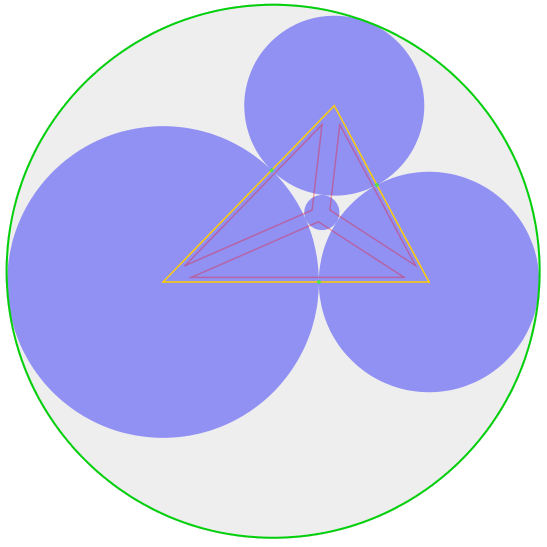
\includegraphics[width=0.65\textwidth]{handleiding-visualisatie-1.png}
  \caption{Voorbeeld visualisatie met drie duidelijke \textit{holes}} \label{fig:handleiding-visualisatie-1}
\end{figure}

\begin{figure}
  \centering
  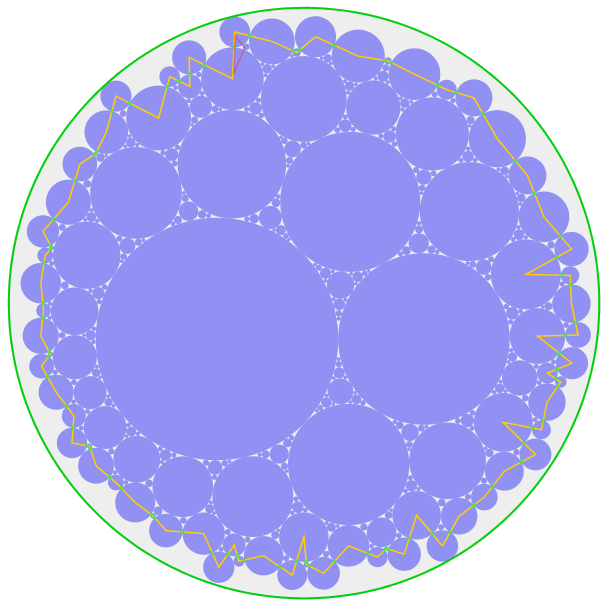
\includegraphics[width=0.65\textwidth]{handleiding-visualisatie-2.png}
  \caption{Voorbeeld visualisatie met grote \textit{shell}} \label{fig:handleiding-visualisatie-2}
\end{figure}

Deze figuren kan u op de volgende manier interpreteren:

\begin{itemize}  
	\item De \textbf{reeds geplaatste cirkels} worden getoond als \textbf{blauwe cirkels}.
	\item De \textbf{shell} is een \textbf{gele lijn} aan de buitenrand van de \textit{packing}. Deze verbindt de middelpunten van de cirkels op de \textit{shell}.
	\item \textbf{Holes} worden getoond als \textbf{rode driehoeken}. De hoekpunten liggen dichtbij de middelpunten van de drie cirkels die de \textit{hole} definiëren.
	\item De \textbf{omschreven cirkel} van de huidige \textit{packing} wordt getoond als een \textbf{groene cirkel}.
\end{itemize}

Merk op dat deze figuren de oorsprong niet als midden hebben, maar steeds gecentreerd zijn rond het midden van de omschreven cirkel van de packing die ze tonen.

Op \autoref{fig:handleiding-visualisatie-1} is zijn er duidelijk drie \textit{holes} te zien.
Elk van de drie \textit{holes} word gedefinieerd door de centrale cirkel en twee van de buitenste cirkels.
Ook is er een kleine \textit{shell} te zien, die bestaat uit de buitenste drie cirkels.
In \autoref{fig:handleiding-visualisatie-2} wordt een verder gevorderde \textit{packing} getoond waarop één \textit{hole} te zien is, en een veel grotere \textit{shell}.
Op beide figuren kan je ook de omcirkel zien.

\chapter{Algoritme} \label{chap:algoritme}

In dit hoofdstuk bespreek ik de werking van de heuristiek.
Eerst geef ik een korte beschrijving van de basis-idee van het algoritme, gevolgd door de structuur van de code.
Vervolgens leg ik stelselmatig de volledige werking uit, samen met alle veronderstellingen die gemaakt worden en geef ik details omtrent implementatie waar nodig.
De volledige implementatie gebeurde in Java, en de broncode is beschikbaar op GitHub \cite{circle-packing-github}.

Om het algoritme zeer snel te maken worden enkele veronderstellingen gemaakt omtrent de nodige overlap-checks bij elke stap.
Deze veronderstellingen zijn niet theoretisch bewezen, maar wel zelf empirisch getest.
Voor de meeste verdelingen van cirkels lijken deze veronderstellingen goed stand te houden, maar er zijn nog enkele \textit{edge-cases} waarin er toch nog fouten gebeuren.
Deze problemen worden besproken in \autoref{chap:bedenkingen} en de snelheid en kwaliteit van de oplossingen wordt verder besproken in \autoref{chap:resultaten}.

\section{Basis-idee}

Het basis-idee van de heuristiek is om stelselmatig een \textit{packing} op te bouwen, door telkens cirkels uit een reeks gegeven cirkels te zoeken die het best passen.
Bij elke stap wordt telkens eerst een positie gekozen om een cirkel te plaatsen in een \textit{hole}, of op de \textit{shell} (zie voor verdere informatie respectievelijk \autoref{sec:holes} en \autoref{sec:shell}).
Hier wordt dan de best-passende cirkel geplaatst, gekozen uit de lijst cirkels die nog geen positie gekregen hebben.
Eenmaal een cirkel geplaatst is wordt deze nooit meer verplaatst.
Dit laat toe om deze \textit{holes} en \textit{shell} efficiënt op te bouwen en gebruiken.
Als de cirkels wel nog verplaatst konden worden zou het veel moeilijker, en rekenintensiever, zijn om deze structuren op te bouwen.
Dan zouden in elke stap alle cirkels met elkaar vergeleken moeten worden om, bijvoorbeeld, te vinden waar nog \textit{holes} zitten.
Zie \autoref{chap:resultaten} voor verdere bespreking van de efficientie van mijn algoritme.

Het algoritme bouwt dus cirkel per cirkel een \textit{packing} op.
Dit gebeurt door in elke stap een positie te kiezen, en hierin een cirkel te proberen plaatsen.
Eerst worden alle \textit{holes} uitgeprobeerd, in de volgorde waarin ze aangemaakt zijn, dan wordt er gekeken naar een plek op de \textit{shell}.
Indien er geen cirkel geplaatst kan worden, wordt de interne structuur van het probleem vernieuwd om deze nieuwe informatie te reflecteren.
Dit gebeurt op verschillende manieren voor de \textit{holes} en de \textit{shell}.
Meer hierover vindt u terug in \autoref{sec:holes} en \autoref{sec:shell}.
Als er wel een cirkel geplaatst kan worden dan wordt deze uit de lijst van nog-te-plaatsen cirkels verwijderd, en krijgt deze een permanente positie op de gekozen locatie.
Het plaatsen van een nieuwe cirkel geeft op zijn beurt ook aanleiding tot aanpassen van de beschikbare \textit{holes} en/of de \textit{shell}.
Hierdoor wordt er een nieuwe tussentijdse \textit{packing} gemaakt.
Deze wordt dan doorgegeven naar de volgende stap, waarin het algoritme opnieuw zal proberen een cirkel te plaatsen.
Op deze manier wordt een volledige \textit{packing} opgebouwd voor alle cirkels.

\section{Structuur van de implementatie}

De implementatie van het algoritme bevat enkele belangrijke (programmeer-)klassen die regelmatig zullen terugkomen in de verdere uitleg, vooral in codefragmenten:

\begin{itemize} 
\item Cirkel (Circle)
\item Vector2
\item Locatie (Location)
\item Probleem (Problem)
\item Oplossing (Solution)
\item Oplosser (Solver)
\item Gat (Hole)
\item Schil (Shell)
\end{itemize}

Een $circle$ is voor de hand liggend. Deze heeft een radius, maar echter geen positie.

$Vector2$ is een 2D positie. Deze bevat een x en y coördinaat.

Een $location$ of locatie is de combinatie van een cirkel met zijn positie. Deze bevat dus een referentie naar een $circle$ en een $vector2$.

Een $problem$ of probleem is een lijst van cirkels.
Deze hebben nog geen positie, en worden gesorteerd van groot naar klein.
Dit is wat de $solver$ als input krijgt.

Een $solution$ of oplossing is een lijst van cirkels met hun positie.
Dit kan een tussenoplossing zijn, waarbij nog niet voor alle cirkels uit een gegeven probleem een positie bestaat.
Ook geeft een solution geen garanties van correctheid, er kan dus bijvoorbeeld overlap zijn. De klasse voorziet echter functionaliteit om dit na te gaan.
Dit is wat de \textit{solver} als output geeft.
Een correcte \textit{solver} geeft natuurlijk wel altijd goede oplossingen.

Een $solver$ of oplosser is het object dat een \textit{packing} zoekt voor een gegeven probleem.
Dit is dus het belangrijkste deel van de code, en hierin is de nieuwe heuristiek geïmplementeerd.
De best-fit \textit{solver}, zoals beschreven in deze thesis, doet dit stap voor stap.
In elke stap wordt er één cirkel geplaats op zijn finale positie, dit aan de hand van enkele keuzes die verder in dit hoofdstuk toegelicht zullen worden.

$Hole$ en $shell$ worden verder uitgelegd in respectievelijk \autoref{sec:holes} en \autoref{sec:shell}.

\section{Structuur van de \textit{solver}}

Zoals hierboven beschreven is de \textit{solver} het hart van de implementatie.
Deze klasse tracht een \textit{packing} te genereren voor een gegeven probleem.
De \textit{solver} bevat een lijst van \textit{holes} en de \textit{shell}.
Hij bevat ook een lijst van de nog te plaatsen cirkels en een tussen-oplossing met de cirkels die reeds een plaats gekregen hebben.
Ook heeft hij een interne omcirkel voor deze oplossing.
Een oplossing kan zelf ook een omcirkel berekenen, maar de \textit{solver} gebruikt een interne omcirkel die enkel vernieuwd wordt wanneer het nodig is.
Bovendien heeft de \textit{solver} extra informatie die de oplossing niet heeft, waardoor deze omcirkel efficiënter berekend kan worden.
Zie \autoref{sec:shell} voor meer uitleg hierover.

In de implementatie ziet de code van de \textit{solver} er als volgt uit (vereenvoudigde versie):

\begin{lstlisting}
List<Circle> circlesToPack; |\label{code:start-vars}|
Queue<Hole> holes;
List<Location> shell;
Location enclosingCircle;

Solution solution; |\label{code:end-vars}|

void solve() { |\label{code:start-solve}|
	init();
	packFirstThree();
	
	while(!circlesToPack.isEmpty()) { |\label{code:best-fit-loop}|
		boolean ok = bestFitStep();
		if (!ok) break;
	}
}

boolean bestFitStep() {
	if (circlesToPack.isEmpty()) {
		return false;
	}
	
	if(!holes.isEmpty()) {
		...
		// Probeer een cirkel in een gat te plaatsen
		...
		return true;
	}
	else if (!shell.isEmpty()) {
		...
		// Probeer een cirkel op de shell te plaatsen
		...
		return true;
	}
}
\end{lstlisting}

De \textit{solver} bevat alle nodige informatie over de \textit{shell} en de \textit{holes}, alsook de cirkels die nog geplaatst moeten worden en de huidige tussen-oplossing (\autoref{code:start-vars} tot \autoref{code:end-vars}).
Om een probleem op te lossen wordt de $solve()$ methode (\autoref{code:start-solve}) aangeroepen.
Deze initialiseert eerst alle nodige variabelen, doet dan de initiële \textit{packing} (meer hierover in \autoref{sec:initialisatie}) en voert dan best-fit-stappen uit tot een oplossing bereikt is (vanaf \autoref{code:best-fit-loop}).

De best-fit \textit{solver} uit deze thesis kan stap voor stap de oplossing genereren en eveneens de tussentijdse oplossingen visualiseren.
Het is dus niet nodig een \textit{packing} volledig te maken en het kan zeer nuttig zijn tussentijdse oplossingen te zien, zeker bij het debuggen of implementeren van nieuwe functionaliteit.

\section{Initialisatie} \label{sec:initialisatie}

Zoals eerder gezegd bouwt het algoritme steeds verder op een \textit{packing} uit de vorige stap.
Hierdoor is het dus nodig om een initiële \textit{packing} te maken van een aantal cirkels waarop de volgende stappen kunnen verderbouwen.
Deze initiële \textit{packing} is de optimale \textit{packing} van de drie grootste cirkels in het probleem.
Deze drie cirkels worden zo geplaatst dat ze alle drie aan elkaar raken, zoals getoond in \autoref{fig:initialisatie}.
De blauwe cirkels tonen de drie cirkels die het eerst geplaatst zijn.
Meer uitleg over interpreteren van deze figuur kan u vinden in \autoref{chap:handleiding-visualisaties}

\begin{figure}
  \centering
  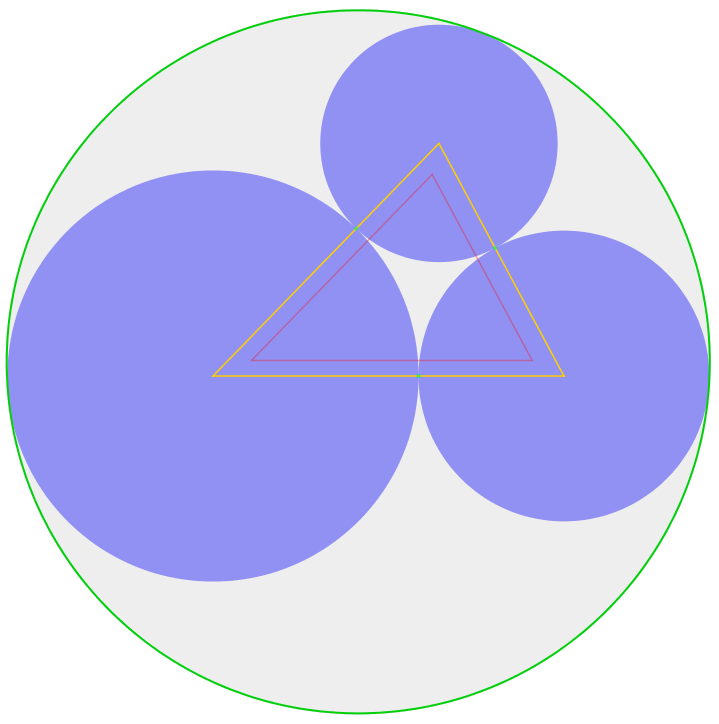
\includegraphics[width=0.65\textwidth]{initialisatie.png}
  \caption{Voorbeeld van initiële \textit{packing}} \label{fig:initialisatie} 
\end{figure}

Het exacte proces om deze initiële \textit{packing} te bekomen wordt verduidelijkt aan de hand van code uit de implementatie:

\begin{lstlisting}
private void packFirstThree() {
	// Plaatst eerst de twee grootste cirkels naast elkaar
	Circle first = circlesToPack.get(0); |\label{code:start-grootste-twee-plaatsen}|
	Circle second = circlesToPack.get(1);

	Vector2 firstPos = new Vector2(0, 0);
	Vector2 secondPos = new Vector2(first.getRadius() + second.getRadius(), 0); |\label{code:end-grootste-twee-plaatsen}|

	Location firstLoc = new Location(firstPos, first);
	Location secondLoc = new Location(secondPos, second);
	getSolution().add(firstLoc); |\label{code:twee-grootste-aan-sol-toevoegen}|
	getSolution().add(secondLoc);
	
	// Plaats de derde grootste cirkel bovenop de eerste twee
	Circle third = circlesToPack.get(2);
	Vector2 thirdPos = Helpers.getMountPositionFor(third, firstLoc, secondLoc); |\label{code:derde-grootste-positie-berekenen}|
	Location thirdLoc = new Location(thirdPos, third);
	getSolution().add(thirdLoc);

	circlesToPack.remove(first);
	circlesToPack.remove(second);
	circlesToPack.remove(third);
	
	// Maak de eerste hole
	holes.add(new NHole(firstLoc, secondLoc, thirdLoc)); |\label{code:eerste-gat-maken}|
	// Maak de initiele shell
	// BELANGRIJK: Deze moeten met-de-klok mee op de shell geplaats worden
	shell.add(firstLoc); |\label{code:initiele-shell-maken}|
	shell.add(thirdLoc);
	shell.add(secondLoc);

	enclosingCircle = Location.calculateEnclosingCircle(Arrays.asList(firstLoc, secondLoc, thirdLoc));
}
\end{lstlisting}

Eerst worden de twee grootste cirkels naast elkaar geplaatst.
Vanaf \autoref{code:start-grootste-twee-plaatsen} tot \autoref{code:end-grootste-twee-plaatsen} worden eerst de twee grootste cirkels uit het probleem opgevraagd.
De lijst \textit{circlesToPack} is gesorteerd van groot naar klein, dus dit zijn de eerste twee cirkels in deze lijst.
De eerste wordt in de oorsprong geplaatst, en de tweede er tegen op de horizontale as.
Deze worden ook reeds aan de tussentijdse oplossing toegevoegd (vanaf \autoref{code:twee-grootste-aan-sol-toevoegen}).
Vervolgens wordt de positie berekend voor de derde cirkel aan de hand van een helper functie op \autoref{code:derde-grootste-positie-berekenen}.
Deze helper functie komt regelmatig terug, en wordt verduidelijkt in \autoref{sec:een-cirkel-tegen-twee-andere-plaatsen}.

In de initialisatie wordt ook de eerste \textit{hole} gemaakt, gedefinieerd door de eerste drie cirkels.
Dit gat wordt toegevoegd aan de lijst van \textit{holes} in de \textit{solver} op \autoref{code:eerste-gat-maken}.
Ook wordt de \textit{shell} aangemaakt, vanaf \autoref{code:initiele-shell-maken}.
Deze wordt met de klok mee (gezien vanuit het centrum van de huidige \textit{packing}) bijgehouden.
Verdere uitleg hierover is te vinden in \autoref{sec:shell}.

\section{Een cirkel tegen twee andere cirkels plaatsen} \label{sec:een-cirkel-tegen-twee-andere-plaatsen}

In verschillende delen van de implementatie is het nodig om een cirkel $c_i$, met radius $r_i$, tegen twee andere cirkels te plaatsen.
Deze twee cirkels noemen we $c_g1, c_g2$, en hun radii $r_g1, r_g2$.
Het punt waarop deze cirkel moet staan om beide andere cirkels te raken wordt bepaald door een eenvoudige cirkel-cirkel intersectie, tussen twee cirkels met hun middelpunt gelijk aan het middelpunt van de cirkels $c_g1$ en $c_g2$ en als radii $r_g1+r_i$ en $r_g2+r_i$:

\begin{lstlisting}
Vector2 getMountPositionFor(Circle cir, Location first, Location second) {
	double x0 = first.getPosition().getX();
	double y0 = first.getPosition().getY();
	double r0 = first.getCircle().getRadius() + cir.getRadius();

	double x1 = second.getPosition().getX();
	double y1 = second.getPosition().getY();
	double r1 = second.getCircle().getRadius() + cir.getRadius();

	// dx en dy zijn de verticale en horizontale afstand tussen de cirkel-centra.
	double dx = x1 - x0;
	double dy = y1 - y0;

	// Bepaal de afstand tussen de centra
	//d = sqrt((dy*dy) + (dx*dx));
	double d = Math.hypot(dx, dy);

	// 'Punt 2' is het punt waar de lijn door de cirkel-intersectie punten de lijn tussen de cirkel-centra kruist
	// We berekenen hier de coordinaten x2 en y2 van dit punt

	// Bepaal eerst de afstand van tussen Punt 2 en het centrum van de eerste cirkel
	double a = ((r0*r0) - (r1*r1) + (d*d)) / (2.0 * d);

	// Bepaal dan de coordinaten van Punt 2.
	double x2 = x0 + (dx * a/d);
	double y2 = y0 + (dy * a/d);

	// Bepaal nu de afstand van Punt 2 naar een van de intersectie-punten
	// Het tweede intersectie-punt ligt even ver
	double h = Math.sqrt((r0*r0) - (a*a));

	// Zet deze afstand om naar een vector met de juiste richting
	double rx = -dy * (h/d);
	double ry = dx * (h/d);

	// Bepaal een van de tweede intersectie punten
	return new Vector2(x2 - rx, y2 - ry); |\label{code:cirkel-cirkel-intersectie-neg}|
}
\end{lstlisting}

In deze code wordt één van de intersectiepunten bepaald.
Dit punt is het punt dat aan uw linker kant zou liggen indien u wandelt van het centrum van de eerste cirkel naar het centrum van de tweede cirkel.
Dit is verduidelijkt in \autoref{fig:cirkel-cirkel-intersectie}, de onderste cirkel is de eerste, de bovenste cirkel de tweede.
De pijl tussen deze cirkels geeft de \textit{wandelrichting} aan.

Ik noem dit intersectiepunt het \textit{negatieve punt}.
Als op \autoref{code:cirkel-cirkel-intersectie-neg} $+$ gebruikt wordt in plaats van $-$ kan het tweede punt bekomen worden, het \textit{positieve punt}.
Het is ook mogelijk het andere intersectie punt te verkrijgen door de twee $location$ parameters om te wisselen.

\begin{figure}
  \centering
  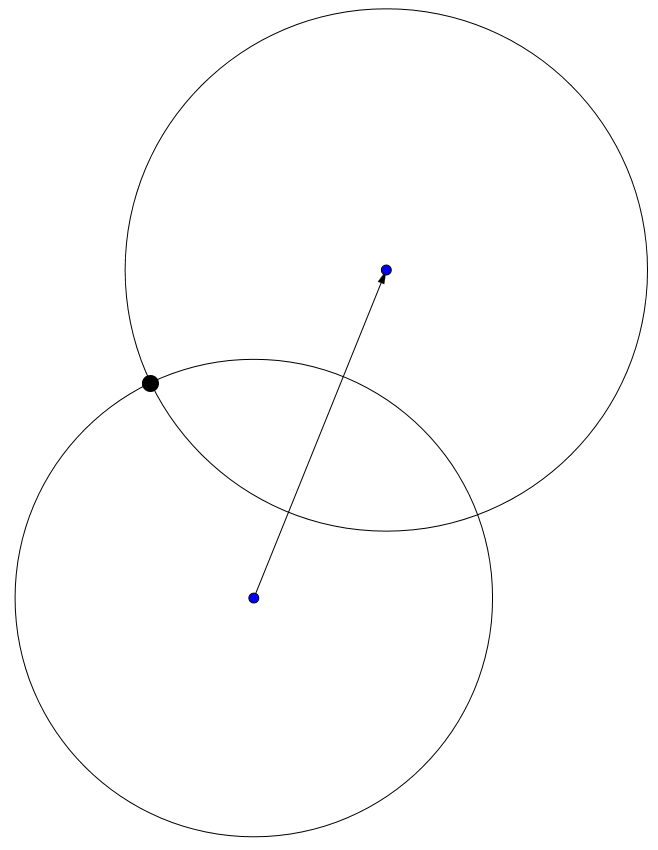
\includegraphics[width=0.65\textwidth]{cirkel-cirkel-intersectie.png}
  \caption{Verkregen intersectie punt van $getMountPositionFor$} \label{fig:cirkel-cirkel-intersectie} 
  \caption*{(Gemaakt met web.geogebra.org)}
\end{figure}

\section{Holes} \label{sec:holes}

Het eerste van de twee belangrijkste concepten van de heuristiek is \textit{holes} of \textit{gaten}.
Dit zijn plaatsen tussen andere, reeds geplaatste, cirkels waar potentieel nog een cirkel kan tussenpassen.
De heuristiek zal telkens eerst deze \textit{holes} proberen op te vullen, alvorens cirkels op de \textit{shell} te plaatsen.
Dit omdat het plaatsen van een cirkel in een \textit{hole} nooit de omschreven cirkel kan vergroten.

\textit{Holes} worden gedefinieerd door exact drie cirkels in de huidige \textit{packing}.
De \textit{solver} houdt informatie bij voor elke \textit{hole} waar mogelijk nog een cirkel in kan passen.
Bij elke stap van de \textit{solver} zal er eerst gekeken worden of er nog \textit{holes} in de oplossing zijn.
Indien er nog \textit{holes} zijn zal het algoritme hier eerst een cirkel in proberen plaatsen.
Indien de \textit{hole} te klein is voor alle nog-te-plaatsen cirkels wordt deze \textit{hole} simpelweg verwijderd uit de lijst van \textit{holes} in de \textit{solver}.
Op deze manier weet de \textit{solver} in de volgende stap dat hij daar niet meer moet proberen om een cirkel te plaatsen, en zal hij een andere \textit{hole} uitproberen.
Indien er wel een cirkel in de \textit{hole} past, wordt deze in de \textit{hole} in geplaatst.
Dit zal leiden tot het creëren van drie nieuwe \textit{holes}, zoals getoond in \autoref{fig:voorbeeld-gat-stap-1} en \autoref{fig:voorbeeld-gat-stap-2}.
De eerste figuur toont de \textit{hole} waarin een cirkel geplaatst zal worden (de rode driehoek).
De tweede figuur toont de nieuwe \textit{packing}, nadat een cirkel geplaatst is in deze \textit{hole}.
Er zijn drie nieuwe kleinere \textit{holes} gemaakt, die in de volgende stappen ook zullen opgevuld worden indien mogelijk.
Het algoritme zal deze \textit{holes} ook terug proberen op te vullen.
In \autoref{fig:voorbeeld-gat-stap-3} en \autoref{fig:voorbeeld-gat-stap-3alt} wordt respectievelijk de tussen-oplossing getoond voor wanneer er nog een cirkel is die klein genoeg is, en wanneer dit niet het geval is, om de onderste \textit{hole} op te vullen.

\begin{figure}
  \centering
  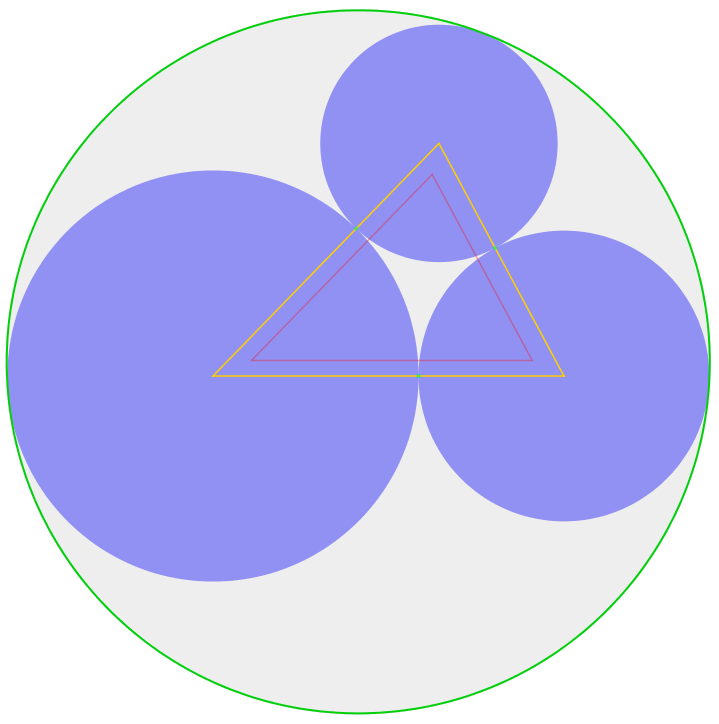
\includegraphics[width=0.65\textwidth]{voorbeeld-gat-stap-1.png}
  \caption{\textit{Packing} voor het opvullen van een \textit{hole}} \label{fig:voorbeeld-gat-stap-1} 
\end{figure}

\begin{figure}
  \centering
  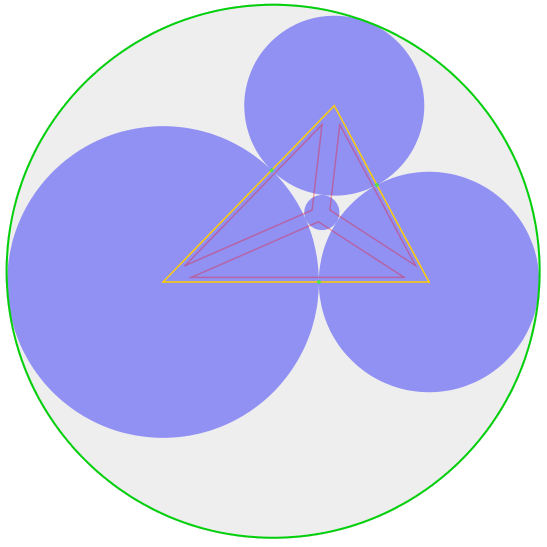
\includegraphics[width=0.65\textwidth]{voorbeeld-gat-stap-2.png}
  \caption{\textit{Packing} na het opvullen van een \textit{hole}} \label{fig:voorbeeld-gat-stap-2} 
\end{figure}

\begin{figure}
  \centering
  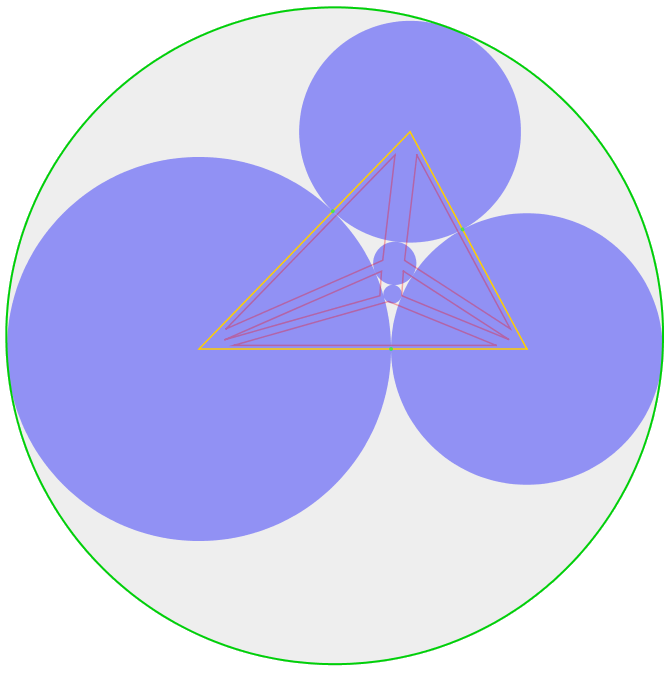
\includegraphics[width=0.65\textwidth]{voorbeeld-gat-stap-3.png}
  \caption{\textit{Packing} na het opvullen van een tweede \textit{hole}} \label{fig:voorbeeld-gat-stap-3} 
\end{figure}

\begin{figure}
  \centering
  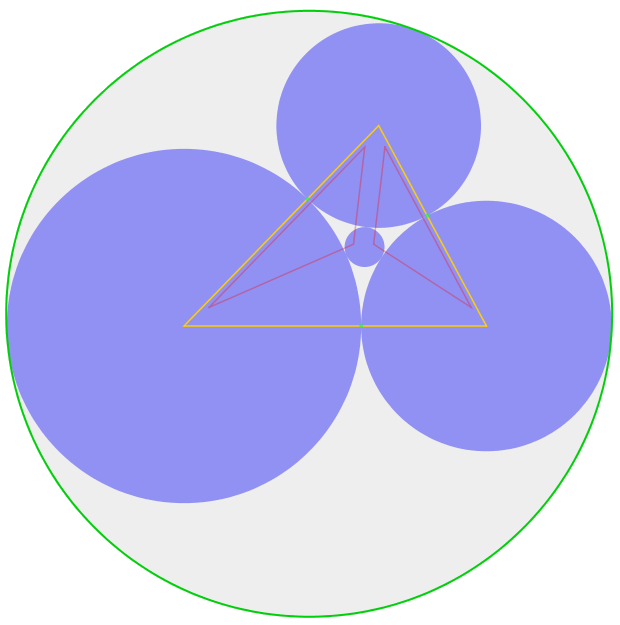
\includegraphics[width=0.65\textwidth]{voorbeeld-gat-stap-3alt.png}
  \caption{\textit{Packing} als het opvullen van een tweede \textit{hole} mislukt} \label{fig:voorbeeld-gat-stap-3alt} 
\end{figure}

\subsection{Grootste cirkel zoeken die past in een \textit{hole}} \label{sec:grootste-cirkel-zoeken-die-past-in-een-hole}

Bij het plaatsen van een cirkel in een \textit{hole} wordt een zo groot mogelijke cirkel gezocht die in deze \textit{hole} past.
Dit is de \textit{best-passende} cirkel, vandaar \textit{best-fit}.
Meer uitleg over hoe bepaald wordt of een cirkel past is terug te vinden \autoref{subsec:bepalen-of-een-cirkel-past-in-hole}.
Hier wordt het proces om te vinden \textit{welke} cirkel past verder verduidelijkt.
Er wordt binair gezocht door de lijst van cirkels om te bepalen welke cirkel de grootste is die past.
Onderstaande code verduidelijkt dit proces.

\begin{lstlisting}
Location findBestFitFor(Hole hole, List<Circle> sortedBigToSmall) {
	// Probeer eerst de kleinste cirkel
	int lower = sortedBigToSmall.size() - 1; |\label{code:probeer-eerst-kleinste-in-hole}|
	Circle smallestCir = sortedBigToSmall.get(lower);
	Vector2 smallestPos = hole.tryFit(smallestCir);
	if (smallestPos == null) {
		return null;
	}

	// Probeer dan de grootste cirkel
	int upper = 0; |\label{code:probeer-dan-grootste-in-hole}|
	Circle biggestCir = sortedBigToSmall.get(upper);
	Vector2 biggestPos = hole.tryFit(biggestCir);
	if (biggestPos != null) {
		return new Location(biggestPos, biggestCir);
	}

	// Binair zoeken
	Circle cir = null;
	Vector2 pos = null;
	while (lower - upper > 1) {
		int middle = (upper + lower) / 2;
		cir = sortedBigToSmall.get(middle);
		pos = hole.tryFit(cir);

		if (pos == null) {
			upper = middle;
		}
		else {
			lower = middle;
		}
	}

	cir = sortedBigToSmall.get(lower);
	pos = hole.tryFit(cir);
	if (pos != null) {
		return new Location(pos, cir);
	}
	else {
		return null;
	}
}
\end{lstlisting}

De \textit{solver} houdt de lijst van cirkels bij gesorteerd op grootte, dat is cruciaal om snel de beste-passende cirkel te vinden.
Eerst worden de grootste en kleinste cirkel uitgeprobeerd (\autoref{code:probeer-eerst-kleinste-in-hole}).
Indien de kleinste niet past zal het algoritme direct rapporteren dat deze \textit{hole} te klein is.
De \textit{hole} zal dan, zoals vermeld in \autoref{sec:holes}, verwijderd worden uit de lijst van mogelijk \textit{holes}.
Indien de grootste past (\autoref{code:probeer-dan-grootste-in-hole}) zal het algoritme onmiddellijk deze cirkel plaatsen in de \textit{hole}.
Er zijn immers geen grotere cirkels, dus deze is de cirkel die verondersteld wordt best te passen.
Vervolgens wordt er een gebied bepaald in de overblijvende cirkels, waarin de best-passende cirkel zich bevindt.
Initieel ligt de boven-en ondergrens van dit gebied op de uiteinden van de overblijvende cirkels.
De cirkel in de midden van dit gebied wordt dan uitgeprobeerd.
Afhangende of deze wel of niet past zal de boven-of ondergrens aangepast worden.
Dit wordt telkens herhaald tot er nog maar één cirkel over blijft.
Dit is dan de grootste cirkel die past, de \textit{best-fit} voor deze \textit{hole}.

\subsection{Bepalen of een cirkel past in een \textit{hole}} \label{subsec:bepalen-of-een-cirkel-past-in-hole}

Er is geen exacte definitie van de grootte van een \textit{hole}.
Dit is niet mogelijk omdat de cirkels die de \textit{hole} bepalen niet altijd aan elkaar raken.
Het is echter wel mogelijk om te bepalen of een cirkel past.

Dit gebeurt door de cirkel die we willen testen te plaatsen in de \textit{hole}.
Eerst wordt de cirkel tegen twee van de cirkels in de \textit{hole} geplaatst, met een cirkel-cirkel intersectie zoals beschreven in \autoref{sec:een-cirkel-tegen-twee-andere-plaatsen}.
Deze cirkel-cirkel intersectie heeft natuurlijk altijd twee punten.
Hiervan moet er één gekozen worden.
De implementatie zorgt er voor dat de cirkels die de \textit{hole} definiëren telkens tegen de klok gesorteerd zijn (ten op zichte van het middelpunt van deze deze drie cirkels).
Dit maakt het mogelijk telkens het juiste punt te kiezen.
Eenmaal dit punt bepaald is word de cirkel op deze plek gezet.
Dan wordt gekeken of deze cirkel wel effectief in de \textit{hole} geplaatst is, en of deze niet overlapt met de derde cirkel die de \textit{hole} definieert.

\begin{lstlisting}
public Vector2 tryFit(Circle cir) {
	// Zoek een positie voor de cirkel
	Vector2 pos = Helpers.getMountPositionFor(cir, first, second);

	// Kijk na of deze positie wel in de hole ligt
	boolean inside = Vector2.isInsideTriableBy(first.getPosition(), second.getPosition(), third.getPosition(), pos); |\label{code:try-fit-in-triangle}|
	if (!inside) {
		return null;
	}

	// Test of er geen overlap is met de derde cirkel
	Location loc = new Location(pos, cir);
	if (third.overlaps(loc)) { |\label{code:try-fit-derde-overlap}|
		return null;
	}
	return pos;
}
\end{lstlisting}

Op \autoref{code:try-fit-in-triangle} wordt verzekerd dat het middelpunt van de cirkel in de \textit{hole} ligt.
Dit voorkomt dat de geplaatste cirkel buiten de \textit{hole} geplaatst wordt, en dus zeker niet kan overlappen met cirkels buiten de \textit{hole} zonder ook te overlappen met één van de cirkels die de \textit{hole} definiëren.
Op \autoref{code:try-fit-derde-overlap} wordt dan de overlap met de derde \textit{hole}-definiërende cirkel nagekeken.
Er kan geen overlap zijn met de eerste twee want de methode $getMountPositionFor$ plaatst de cirkel zodanig dat deze de twee andere cirkels raakt, maar niet overlapt.
Indien de cirkel in de \textit{hole} past, en dus alle checks doorstaat, wordt de positie voor deze cirkel teruggegeven.
De \textit{solver} zal deze cirkel dan in zijn oplossing plaatsen.

Het is niet nodig om na te gaan of er overlap is met andere cirkels in de oplossing.
Als er met een andere overlap zou zijn, moet dit zijn omdat de cirkel buiten de \textit{hole} geplaatst is, of er is ook overlap met één van de cirkels in de \textit{hole} zelf.
Dit zorgt er voor dat er zeer weinig overlap-checks gedaan moeten worden, wat het algoritme zeer snel maakt.

\section{Shell} \label{sec:shell}

De \textit{shell} of \textit{schil} is het tweede belangrijke concepten in de heuristiek.
Dit is de buitenste laag van cirkels in een (tussen-)oplossing van de \textit{solver}.
Deze wordt in de implementatie bijgehouden als een geordende lijst van cirkels.
Cirkels die naast elkaar staan in de lijst, grenzen ook aan elkaar in de \textit{shell}.
De cirkels in deze laag zijn met de klok mee gesorteerd, ten opzichte van het middelpunt van de omcirkel.
De eerste en laatste cirkel in de lijst volgen elkaar ook op in de \textit{shell}, en er is dus geen echt begin of einde van de \textit{shell}.

De heuristiek voorgesteld in deze thesis probeert steeds eerst alle \textit{holes} op te vullen.
Maar wanneer er geen cirkels meer over zijn die klein genoeg zijn om te passen in \textit{holes}, wordt er een cirkel op de \textit{shell} geplaatst.
Op de \textit{shell} worden alle posities tegen twee cirkels van de \textit{shell} overwogen.
Deze aanpak beperkt het aantal mogelijke posities voor de geplaatste cirkel enorm en maakt het algoritme dus zeer snel (zie \autoref{chap:resultaten} voor een vergelijking in snelheid).
Er wordt steeds een cirkel zo dicht mogelijk bij het centrum van de huidige tussen-oplossing geplaatst.
Dit om het uitbreiden van de omschreven cirkel zo min mogelijk te houden en dus een nieuwe tussen-oplossing te bekomen die zo goed mogelijk is.

Eerst worden twee cirkels gekozen waartegen de nieuwe cirkel geplaatst zal worden.
Hiervoor wordt gekeken naar het middelpunt tussen alle cirkels die naast elkaar staan op de \textit{shell}.
De twee cirkels waarvoor het middelpunt het dichtst bij het centrum van de huidige omschreven cirkel ligt, worden gekozen als kandidaten om de derde cirkel tegen te plaatsen.
Dan wordt er gezocht naar een zo groot mogelijke cirkel die daar past op de \textit{shell}.

Indien geen enkele cirkel, past wordt één van de twee kandidaat cirkels verwijderd uit de \textit{shell}.
Welke verwijderd wordt is verduidelijkt in \autoref{sec:bepalen-of-een-cirkel-past-op-de-shell}.
Dit zorgt er voor dat de \textit{shell} verandert en \textit{groeit} naar buiten.
In de volgende stap van het algoritme zal dan ook een andere positie voor een cirkel uitgeprobeerd worden.

Indien er wel een cirkel past, wordt deze toegevoegd aan de \textit{shell}, en geeft deze aanleiding tot een nieuwe \textit{hole}.
Deze \textit{hole} zal vervolgens opgevuld worden indien mogelijk, zoals beschreven in \autoref{sec:holes}.
Op \autoref{fig:plaats-op-shell-simpel} wordt getoond hoe de \textit{packing} verandert wanneer een cirkel geplaatst wordt op de \textit{shell}.
Eerst wordt een \textit{packing} zonder \textit{holes} getoond en vervolgens de \textit{packing} nadat een cirkel op de \textit{shell} geplaatst is.
Hierop is duidelijk te zien hoe de \textit{shell} aangepast werd, en deze plaatsing geleid heeft tot een nieuwe \textit{hole}.
De gele lijn, die de \textit{shell} voor stelt, verbindt nu één extra cirkel, en de rode driehoek toont de nieuwe \textit{hole}.

Zoals eerder aangegeven is het mogelijk dat de grootste cirkel niet past op deze positie op de \textit{shell}.
Het algoritme zal dan proberen een (beschikbare) kleinere cirkel op de \textit{shell} te plaatsen, dit wordt geïllustreerd in \autoref{fig:plaats-op-shell-kleiner}.
Het is ook mogelijk dat geen enkele cirkel past op de positie in de \textit{shell} die het dichts bij het centrum van de huidige omschreven cirkel ligt.
Dit wordt getoond in \autoref{fig:plaats-op-shell-geen-enkele-past}.
Dan zal de \textit{shell} uitgebreid worden naar buiten, en zal in de volgende stap van het algoritme een andere positie op de \textit{shell} uitgeprobeerd worden.

\begin{figure}
  \centering
  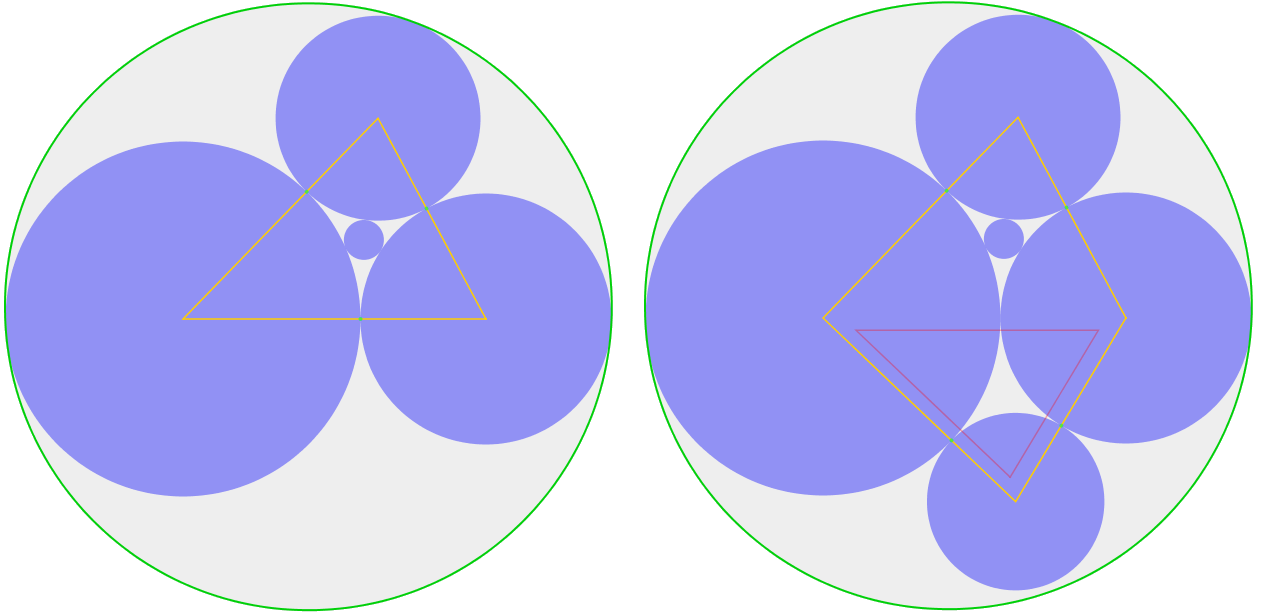
\includegraphics[width=1.0\textwidth]{plaats-op-shell-simpel.png}
  \caption{Het plaatsen van de grootste cirkel op de \textit{shell}} \label{fig:plaats-op-shell-simpel} 
\end{figure}

\begin{figure}
  \centering
  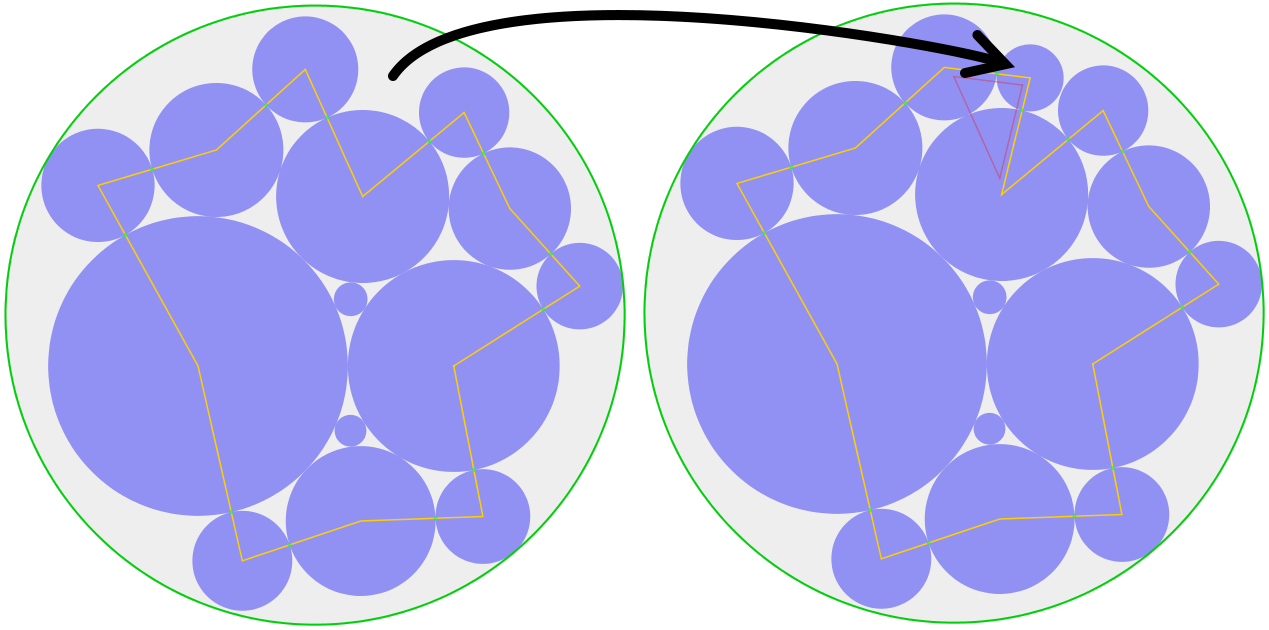
\includegraphics[width=1.0\textwidth]{plaats-op-shell-kleiner_arrow.png}
  \caption{Het plaatsen van een kleinere cirkel op de \textit{shell}} \label{fig:plaats-op-shell-kleiner}
\end{figure}

\begin{figure}
  \centering
  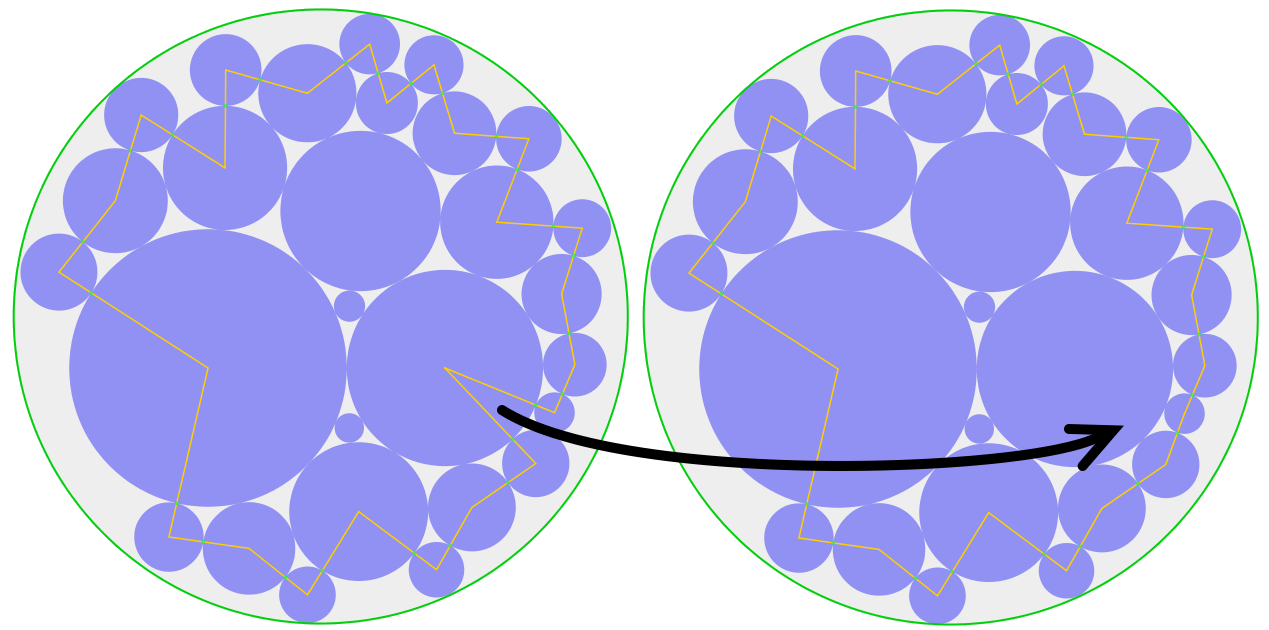
\includegraphics[width=1.0\textwidth]{plaats-op-shell-geen-enkele-past_arrow.png}
  \caption{\textit{Shell} aanpassen als geen enkele cirkel past} \label{fig:plaats-op-shell-geen-enkele-past}
\end{figure}

\subsection{Efficienter de omcirkel berekenen gebaseerd op de \textit{shell}}

Bij het kiezen van de kandidaat-cirkels om een cirkel tegen te plaatsen op de \textit{shell} wordt gebruik gemaakt van de omschreven cirkel van de huidige tussen-oplossing.
Zoals eerder vermeld kan voor elke (tussen-)oplossing de omcirkel berekend worden.
Dit gebeurt door een aangepaste versie van het Welz algoritme voor de omcirkel van punten beschreven in \cite{welzl1991smallest}.
De gebruikte implementatie is gebaseerd op de implementatie in \cite{sunshine2008welzl}.
Het is een recursief algoritme dat in lineaire tijd de omcirkel kan berekenen.
Het basisidee bestaat eruit dat de omcirkel van een aantal cirkels (of punten) volledig gedefinieerd is door maximum drie van deze cirkels.
Het algoritme vindt deze cirkels uit een gegeven lijst cirkels.

Het is intuïtief te begrijpen dat deze cirkels aan de buitenkant van een oplossing zullen liggen.
Dat is ook net waaruit de \textit{shell} bestaat, de cirkels aan de buitenkant van een oplossing.
Het is dus mogelijk om in elke stap van de \textit{solver} de omcirkel zeer efficiënt te berekenen.
De complexiteit is dan slechts lineair in het aantal cirkels op de \textit{shell} van de huidige (tussen-)oplossing, wat slechts een subset is van het totaal aantal cirkels in de oplossing.
Aangezien de omcirkel regelmatig moet worden herberekend  doorheen het algoritme is dit een zeer interessante optimalisatie.

\subsection{Bepalen of een cirkel past op de \textit{shell}} \label{sec:bepalen-of-een-cirkel-past-op-de-shell}

Om te bepalen of een cirkel op de \textit{shell} past, plaatsen we de cirkel eerst tegen twee cirkels op de \textit{shell}.
Dit gebeurt op dezelfde manier als het plaatsen van een cirkel tegen twee cirkels van een \textit{hole}.
De exacte methode is reeds uiteengezet in \autoref{sec:een-cirkel-tegen-twee-andere-plaatsen}.
Eenmaal deze positie gekend is, wordt er nagekeken of dit niet tot overlap leidt.
Indien er overlap is, is het niet mogelijk om de cirkel daar op de \textit{shell} te plaatsen en wordt er informatie terug gegeven over welke cirkel op de \textit{shell} voor problemen zorgt.

Om na te gaan of er overlap is, worden er systematisch een aantal cirkels op de \textit{shell} nagekeken.
Het is niet nodig andere cirkels, die niet op de \textit{shell} zitten, na te kijken voor overlap.
Dat is zo omdat een nieuwe cirkel steeds op de \textit{shell} geplaatst wordt zodanig dat als er overlap zou zijn met cirkels in de oplossing, minstens één van die cirkels op de \textit{shell} ligt.
Omdat ik geen exacte wiskundige definitie van de \textit{shell} heb (de \textit{shell} is enkel gedefinieerd door het algoritme dat ze opbouwt) is het niet mogelijk om hier een echt bewijs van te geven.
Uit eigen empirische tests blijkt de verwachting omtrent deze overlappingen echter wel te kloppen.
Verdere bedenkingen hierbij zijn terug vinden in \autoref{chap:bedenkingen}.
Om deze overlappingstest zo snel mogelijk te kunnen uitvoeren, worden eerst cirkels dichtbij op de \textit{shell} nagekeken.
Er staat ook een limiet op het aantal cirkels dat getest wordt.
Uit tests, tot 5000 cirkels, blijkt dat drie cirkels aan elke kant van de \textit{shell} nakijken genoeg is.
Voor de meeste gevallen is één cirkel nakijken genoeg, maar sommige randgevallen (wanneer meerdere kleine cirkels dichtbij elkaar staan op de \textit{shell}) vragen deze extra checks.

Het aantal cirkels dat nagekeken wordt is een hyperparameter $checkRadius$ van het algoritme.
De volgende code toont hoe de overlap nagekeken wordt:

\begin{lstlisting}
for (int i = 1; i <= checkRadius; ++i) {
	int prevIndex = (firstIndex + shell.size() - i) % shell.size();
	Location prev = shell.get(prevIndex);
	if (loc.overlaps(prev)) {
		toRemove = first;
		break;
	}
	int nextIndex = (secondIndex + i) % shell.size();
	Location next = shell.get(nextIndex);
	if (loc.overlaps(next)) {
		toRemove = second;
		break;
	}
}
\end{lstlisting}

Er wordt dus om te beurt links en rechts van de huidige positie op de \textit{shell} nagekeken voor overlap.
Indien er overlap gevonden is, wordt bijgehouden aan welke kant van de \textit{shell} dit gebeurd is.
$toRemove$ is dus uiteindelijk $first$ of $second$, wat aangeeft of er aan de kant van de eerste cirkel, of van de tweede cirkel, overlap voorkomt.
$toRemove$ kan ook $null$ zijn indien er geen overlap is.
Deze informatie wordt dan gebruikt door de \textit{solver} om te bepalen of de cirkel geplaatst kan worden ($toRemove = null$), of dat de \textit{shell} aangepast moet worden. Deze stap wordt hieronder besproken in \autoref{sec:een-cirkel-plaatsen-op-de-shell}.

\subsection{Een cirkel plaatsen op de \textit{shell}} \label{sec:een-cirkel-plaatsen-op-de-shell}

Om een cirkel op de \textit{shell} te plaatsen wordt eerst de grootste cirkel die op de \textit{shell} past binair gezocht in de lijst van nog-te-plaatsen cirkels.
De gebruikte methode is vergelijkbaar met het zoeken naar de grootste cirkel die past in een \textit{hole}, zoals beschreven in \autoref{sec:grootste-cirkel-zoeken-die-past-in-een-hole}.
Indien er een cirkel gevonden wordt die past op de \textit{shell} wordt de \textit{shell} uitgebreid met deze cirkel.
De cirkel wordt dan tussen de cirkels, waartegen hij geplaatst is, in de \textit{shell} (voorgesteld als lijst) geplaatst.
Dit wordt geïllustreerd in \autoref{fig:plaats-op-shell-simpel}, \autoref{fig:plaats-op-shell-kleiner}.
De gele lijn (die de \textit{shell} voorstelt, zoals beschreven in \autoref{chap:handleiding-visualisaties}) wordt uitgebreid met een extra punt.
Dit zorgt er ook voor dat een nieuwe \textit{hole} gemaakt wordt waar mogelijk kleinere cirkels in passen.

Een laatste check gaat na of door het plaatsen van de cirkel de \textit{shell} nog juist gevormd is.
Indien een cirkel geplaatst wordt zodat de cirkels niet meer met de klok mee gesorteerd zijn, zou dit ervoor kunnen zorgen dat foutieve plaatsingen voorkomen.
Om dit te voorkomen wordt de gerichte hoek tussen de geplaatste cirkel en de cirkels waartegen hij geplaatst is nagekeken.
Indien deze hoek negatief is wordt de \textit{shell} hieraan aangepast.
Dit wordt getoond in \autoref{fig:plaats-op-shell-hoek}.
Het eerste deel toont de configuratie waarop een cirkel geplaatst zal worden.
Het laatste deel de uiteindelijke configuratie van de \textit{shell}.
Het middelste deel toont met een zwarte lijn het deel van de \textit{shell} dat verwijderd is om er voor te zorgen dat deze kloksgewijs gesorteerd blijft.
Op \autoref{fig:plaats-op-shell-hoek-fout}  wordt getoond wat er kan gebeuren als deze check niet gebeurt.
De cirkels worden doorzichtich getekend, het donker-blauwe deel toont dus overlappende cirkels.

\begin{figure}
  \centering
  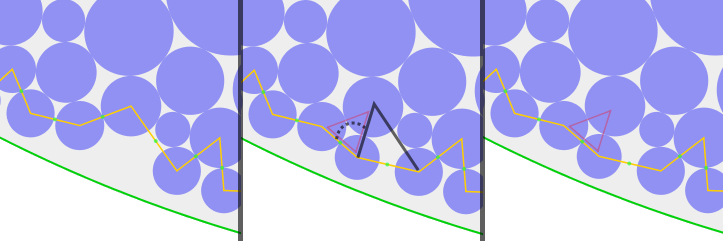
\includegraphics[width=1.0\textwidth]{plaats-op-shell-hoek.png}
  \caption{Een cirkel veroorzaakt een tegen-de-klok \textit{shell}} \label{fig:plaats-op-shell-hoek} 
\end{figure}

\begin{figure}
  \centering
  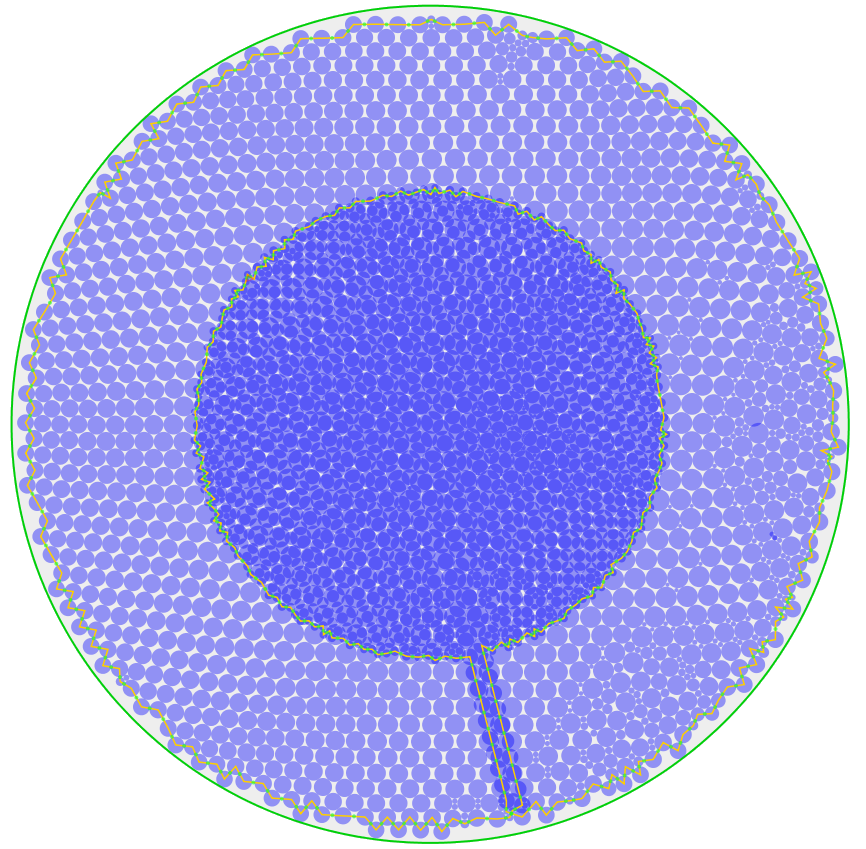
\includegraphics[width=.65\textwidth]{plaats-op-shell-hoek-fout.png}
  \caption{Mogelijke fout indien de \textit{shell} niet met de klok mee gesorteerd is} \label{fig:plaats-op-shell-hoek-fout} 
\end{figure}

\section{Conclusie}

Dit hoofdstuk gaf een volledig overzicht van de nieuwe constructieve heuristiek.
Waar nodig werd de uitleg verduidelijkt met code uit de implementatie.
Er werden ook de verschillende veronderstellingen geformuleerd die gebruikt worden om het algoritme zeer snel te maken.
Zie ook \autoref{chap:bedenkingen} voor verdere bedenkingen hieromtrent.


\chapter{Bedenkingen bij implementatie} \label{chap:bedenkingen}

\section{Precisie}

De implementatie gebruikt $double$ variabelen.
Ook geeft de methode gebruikt om cirkels tegen elkaar te plaatsen, beschreven in \autoref{sec:een-cirkel-tegen-twee-andere-plaatsen}, geen exacte oplossing.
Deze posities worden gebruikt om cirkels te plaatsen, en later worden tegen deze cirkels nieuwe cirkels geplaatst.
Hierdoor wordt er doorheen het algoritme dus een kleine fout opgebouwd.
Deze fout uit zich in een kleine overlap tussen cirkels in de uiteindelijke verkregen \textit{packing}.
Deze overlap blijft echter beperkt tot $10^{-15}$ vierkante eenheden voor de grootste \textit{packings}.

Dit is een inherent probleem van werken in eindige precisie.
Andere algoritmen hebben dus te kampen met hetzelfde probleem, hoewel er niet altijd aandacht aan wordt besteed in de gepubliceerde papers.
In \cite{akeb2006basic}, \cite{ye2013iterated} en \cite{m2013packing} worden resultaten verkregen met een precisie van respectievelijk $10^{-10}$, $10^{-28}$ en $10^{-7}$.

Aangezien de vergelijkingen in \autoref{chap:resultaten} tot een precisie van $10^{-10}$ gebeuren heeft dit verder geen impact op de resultaten.

\section{Veronderstellingen}

Zoals eerder vermeld worden er bij de uitleg over de \textit{holes} en de \textit{shell} enkele veronderstellingen gedaan om het algoritme zeer snel te laten werken.
Deze veronderstellingen lijken voor de meeste problemen correct te zijn.
Er zijn echter sommige problemen, vooral als er gewerkt wordt met zeer hoge aantallen cirkels (duizenden), die wél significante fouten kunnen opleveren.
Deze uiten zich dan in \textit{packings} met een grote overlap.

Uit huidige tests blijkt er vooral een probleem met de \textit{holes}, de \textit{shell} heeft voor zover mijn huidige tests uitwijzen geen problemen.
Doordat de cirkels die een \textit{hole} definiëren niet altijd aan elkaar raken kan het gebeuren dat er toch nog een overlap is, als twee \textit{holes} naast elkaar staan.

Een voorstel om dit op te lossen is een \textit{hole} niet op te delen in drie \textit{holes} als er een cirkel in geplaatst wordt, maar slechts in twee.
Eén van die \textit{holes} bestaat dan uit meer dan drie cirkels.
Zo is het wel mogelijk om altijd aaneensluitende cirkels een \textit{hole} te laten bepalen.
Dit is een oplossing die mogelijk geëxploreerd kan worden in de toekomst, maar wegens tijdsbeperkingen geen deel is van deze thesis.

\chapter{Resultaten} \label{chap:resultaten}

In dit hoofdstuk worden de verkregen \textit{packings} vergeleken met een reeks gekende \textit{packings}, zoals gerapporteerd op de Packomania website \cite{packomania}.
Packomania is een website die de beste oplossingen (in radius van omschreven cirkel) voor verschillende \textit{circle-packing} problemen probeert te verzamelen.
De oplossingen worden onderling vergeleken, op zowel de verkregen radius van de omschreven cirkel, als ook de tijd nodig om tot deze \textit{packing} te komen indien deze gekend is.
De nodige rekentijd voor deze algoritmen is echter niet altijd even makkelijk te vinden.
Veel van de \textit{packings} op Packomania hebben geen bijhorende publicatie.
Het gebruikte algoritme en de nodige tijd om de \textit{packing} te bekomen is dus niet gekend, enkel de verkregen omschreven cirkel en coördinaten van de \textit{packing}.
De vergelijking in tijd zal dus een zeer ruwe vergelijking zijn gebaseerd op slechts enkele papers.

Ook geef ik resultaten voor \textit{packings} met veel meer cirkels dan deze geraporteerd op Packomania.
Hiervoor heb ik geen andere resultaten gevonden in de literatuur om mee te vergelijken.

Packomania heeft resultaten voor verschillende verdelingen van cirkels.
Deze verdelingen zijn als volgt:

\begin{itemize}
	\item $r_i=1$ (alle cirkels gelijke grootte)
	\item $r_i=i$
	\item $r_i=i^{1/2}$
	\item $r_i=i^{-1/5}$
	\item $r_i=i^{-1/2}$
	\item $r_i=i^{-2/3}$
\end{itemize}

Hierbij zijn er telkens $N$ cirkels in het probleem, en is $i \in (1,2,...,N)$.

De laatste vier verdelingen hebben een vaste structuur: $r_i=i^X$.
Hier is $X$ steeds een andere macht.
Deze problemen verzamelen ik onder één noemer: de \textit{Packomania macht} problemen.

De verhouding tussen enkele van deze verdelingen worden verduidelijkt in \autoref{fig:packomania-verdelingen}.

\begin {figure}
	\centering
	\resizebox {0.8\columnwidth} {!} {
		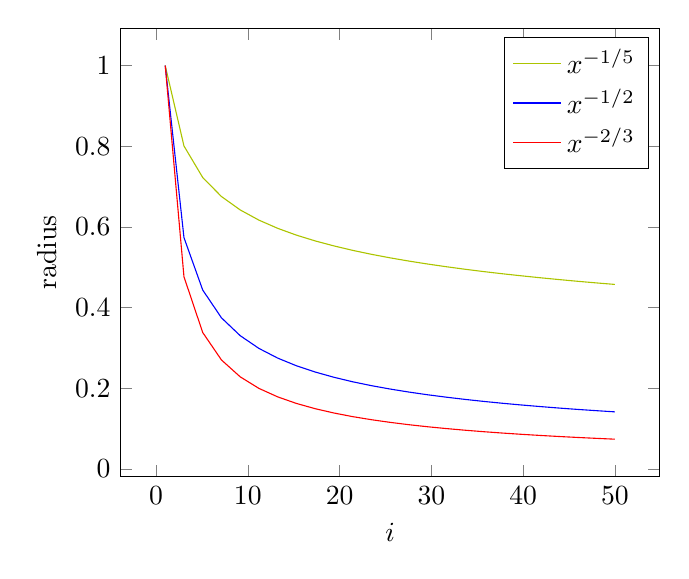
\begin{tikzpicture}
			\begin{axis}[ xlabel=$i$, ylabel=radius, domain=1:50 ]
				\addplot[green]{x^(-1/5)};
				\addlegendentry{$x^{-1/5}$}
				
				\addplot[blue]{x^(-1/2)};
				\addlegendentry{$x^{-1/2}$}
				
				\addplot[red]{x^(-2/3)};
				\addlegendentry{$x^{-2/3}$}
			\end{axis}
		\end{tikzpicture}
	}
	\caption{Packomania verdelingen}
	\label{fig:packomania-verdelingen}
\end {figure}

Al deze berekeningen zijn uitgevoerd op een Mid 2009 Macbook-Pro 15 inch met een 2.8Ghz Core 2 Duo processor en 4GB ram.

\section{Packomania vergelijking}

\subsection{Cirkels met gelijke grootte}

In \autoref{fig:vergelijking-even-grote-cirkels} wordt de procentuele vergroting weergegeven voor \textit{packings} met $N$ cirkels van gelijke grootte.
Er wordt een volledig beeld gegeven, als ook een gedetailleerder beeld waar vergrotingen boven de 1,5\% niet worden weergegeven.
Deze vergroting is afgemeten ten opzichte van de best gekende oplossing op de Packomania website.
Tabellen die mijn resultaten vergeleken met de best gekende tonen zijn terug te vinden in \autoref{append:packomania-tabellen-gelijke-grootte}.

\begin {figure}
	\centering
	\resizebox {0.8\columnwidth} {!} {
		\begin{tikzpicture}
			\begin{axis}[xlabel=Aantal Cirkels, ylabel=\% Vergroting]
				\addplot table [x=N, y=Increase, col sep=comma]{csv/Equal size Packomania problems comparison.csv};
				\addlegendentry{Gelijke grootte}
			\end{axis}
		\end{tikzpicture}
	}
	\resizebox {0.8\columnwidth} {!} {
		\begin{tikzpicture}
			\begin{axis}[xlabel=Aantal Cirkels, ylabel=\% Vergroting, ymin=0, ymax=1.5]
				\addplot table [x=N, y=Increase, col sep=comma]{csv/Equal size Packomania problems comparison.csv};
				\addlegendentry{Gelijke grootte}
			\end{axis}
		\end{tikzpicture}
	}
	\caption{Vergelijking van \textit{packings} van even grote cirkels}
	\label{fig:vergelijking-even-grote-cirkels}
\end {figure}

Gemiddeld geeft mijn algoritme een resultaat dat $0,79\%$ groter is dan het best gekende resultaat voor problemen met cirkels van gelijke grootte.
Er is echter een duidelijke neerwaartse trend.
Voor problemen met meer dan 1000 cirkels is de gemiddelde vergroting nog slechts 0,48\%.
Voor meer dan 2000 cirkels nog 0,39\% en voor meer dan 3000 nog 0,32\%.
Problemen met een groter aantal cirkels geven duidelijk een beter resultaat.

Dit komt mogelijk omdat hoe meer cirkels er zijn, hoe moeilijker het probleem wordt.
Hierdoor zullen de best gekende oplossingen voor problemen met zulke grote aantallen cirkels minder dichtbij de absolute optimale oplossing liggen.
Omdat mijn algoritme enkel nieuwe cirkels tegen twee reeds geplaatste cirkels plaatst, hebben al mijn oplossingen voor dit probleem een duidelijke structuur.
Deze structuur is een zeshoekige structuur.
Dit wordt geïllustreerd in \autoref{fig:packing-even-groot-500}.
Dit is een zeer eenvoudige structuur, maar benaderd redelijk goed de best gekende oplossingen.
Meer figuren hiervan zijn terug te vinden in \autoref{append:extra-packing-figuren}.

De benodigde tijd om tot een oplossing te komen blijft onder 10 milliseconden tot $N=100$.
Tot 500 cirkels blijft de nodige rekentijd onder 100 milliseconden.
De rekentijd loopt pas op tot één seconde bij 2200 cirkels, en slechts 3,5 seconden voor 5000 cirkels.

Zoals eerder vermeld zijn vergelijkingen van berekeningstijden moeilijk te vinden.
In \cite{grosso2010} worden echter tijden gerapporteerd van 110 seconden voor 30 cirkels (mijn algoritme gebruikte hier minder dan een milliseconde), en 15311 seconden (meer dan 4 uur) voor 100 cirkels (mijn algoritme gebruikte voor hetzelfde probleem 7 milliseconden).
Zij halen resultaten die zeer dichtbij de best gekende liggen (soms de beste).

Zelfs de constructieve algoritmen beschreven in \cite{akeb2006basic} en \cite{hifi2004approximate} vragen meerdere seconden, en soms minuten, om te berekenen.
Hun resultaten zijn echter moeilijk te vergelijken omdat \cite{akeb2006basic} een alternatieve versie van \textit{circle-packing} oplost, en \cite{hifi2004approximate} \textit{packings} maakt in rechthoeken.

\begin{figure}
  \centering
  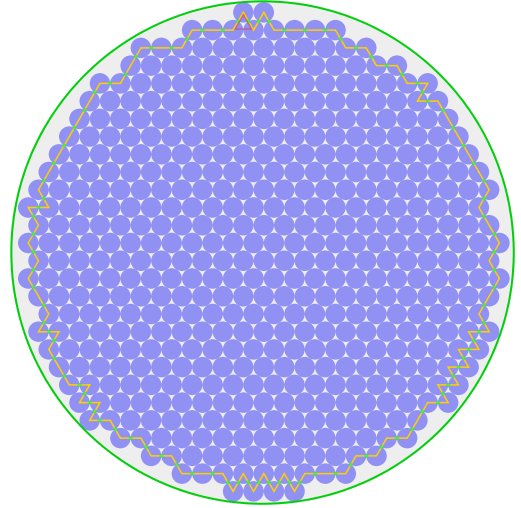
\includegraphics[width=0.65\textwidth]{packing-even-groot-500.png}
  \caption{\textit{Packing} voor 500 even grote cirkels} \label{fig:packing-even-groot-500} 
\end{figure}

\subsubsection{Bespreking}

Over het algemeen zijn dit goede resultaten.
Ze liggen behoorlijk dicht bij de best gekende oplossing, maar hebben een duidelijk en eenvoudig patroon.
Dit patroon is duidelijk te zien in \autoref{fig:packing-even-groot-500}, en is eenvoudig te genereren.
Dit zijn dus zeker niet de meest indrukwekkende resultaten.
Het probleem waar alle cirkels een gelijke grootte hebben is dan ook niet de kracht van mijn algoritme.
Aangezien elke cirkel even groot is, zal er nooit een cirkel gevonden worden die in een \textit{hole} past.
Ook is dit het eenvoudigste probleem.
Het feit dat er resultaten te vinden zijn tot 5000 cirkels op Packomania, maar problemen met verschillende radii slechts tot maximum 200 cirkels opgelost zijn, wijst hier op.
Hoewel mijn algoritme dus relatief goede resultaten geeft voor dit probleem, zijn de resultaten die volgen interessanter.

\subsection{Packomania Benchmark}

Packomania geeft ook resultaten voor enkele benchmark instanties. Deze benchmarks werden geïntroduceerd door WenQi Huang in verscheidene papers, en samengevat in \cite{huang2006new}.
De radii van de cirkels in deze benchmark instanties zijn terug te vinden in \autoref{append:packomania-benchmark-verdelingen}.
Een eerste set verdelingen (met prefix $NR$) heeft tussen 10 en 60 cirkels per probleem, een tweede set (met prefix $IN$) tussen 9 en 28 cirkels met nog één probleem van 162 cirkels.
In elke verdeling zitten cirkels met verschillende raddii, maar ook cirkels met gelijke raddii.

In \autoref{fig:vergelijking-packomania-benchmark} wordt de procentuele vergroting van de oplossing van mijn algoritme vergeleken met de best gekende oplossing.
Gemiddeld geeft mijn algoritme een resultaat dat $5,94\%$ groter is dan de best gekende resultaten.
Door het zeer gelimiteerd aantal instanties is er echter geen duidelijke trend te zien zoals bij \textit{packings} voor cirkels met gelijke grootte, en de Packomania Macht problemen (zie \autoref{sec:vergelijking-packomania-machten}).

\begin {figure}
	\centering
	\resizebox {0.8\columnwidth} {!} {
		\begin{tikzpicture}
			\begin{axis}[xlabel=Aantal Cirkels, ylabel=\% Vergroting]
				\addplot table [x=N, y=Increase, col sep=comma,
						skip coords between index={24}{1000}
					]{csv/IN NR Packomania problems comparison.csv};
				\addlegendentry{NR}

				\addplot table [x=N, y=Increase, col sep=comma,
						skip coords between index={0}{24}
					]{csv/IN NR Packomania problems comparison.csv};
				\addlegendentry{IN}
			\end{axis}
		\end{tikzpicture}
	}
	\caption{Vergelijking van Packomania Benchmark problemen}
	\label{fig:vergelijking-packomania-benchmark}
\end {figure}

De benodigde rekentijd bedraagt voor al deze problemen ook slechts enkele milliseconden.
In \cite{ye2013iterated} worden deze problemen opgelost in tijden tussen 1 seconde voor 10 cirkels, en meer dan 2 uur voor 60 cirkels.
Ook in \cite{huang2013tabu} kan de nodige tijd oplopen tot meerdere uren voor de grotere problemen.
Zelfs de kleinere problemen (10 tot 15 cirkels) kunnen meerdere minuten vragen om berekend te worden.
Mijn algoritme heeft slechts enkele miliseconden nodig voor dezelfde problemen.

\subsubsection{Bespreking}

Ook deze resultaten zijn over het algemeen goed.
Gemiddeld is er slechts een $5,94\%$ vergroting van de radius van de omschreven cirkel, met slechts 3 van de 38 problemen die meer dan $10\%$ vergroting hebben.
Er zijn echter ook 2 problemen die even goed opgelost worden dan de best gekende.

Dit zijn dus goede resultaten, maar het aantal probleeminstanties blijft zeer beperkt.
In de volgende sectie wordt de kracht van dit nieuwe algoritme duidelijker met meer cirkel-verdelingen.

\subsection{Packomania Machten} \label{sec:vergelijking-packomania-machten}

Zoals eerder vermeld neem ik enkele van de Packomania problemen onder één noemer: de \textit{Packomania macht} problemen.
Dit zijn de verdelingen met een vaste structuur: $r_i=i^X$.
Hier is $X \in {1/2, -1/5, -1/2, -2/3}$.
Tabellen die mijn resultaten met de best gekende vergelijken zijn terug tes vinden in \autoref{append:packomania-tabellen-macht}.

In \autoref{fig:vergelijking-packomania-macht} worden voor al deze macht problemen de procentuele vergroting getoond.
Dit is de omtrek van de omschreven cirkel verkregen uit mijn algoritme ten opzichte van de best gekende oplossingen.

\begin {figure}
	\centering
	\resizebox {0.8\columnwidth} {!} {
		\begin{tikzpicture}
			\begin{axis}[xlabel=Aantal Cirkels, ylabel=\% Vergroting, no markers]
				\addplot+[line width=1, opacity=0.5] table [x=N, y=Increase, col sep=comma,
							skip coords between index={196}{10000}
						]{csv/Power Packomania Problems Comparison.csv};
				\addlegendentry{$r_i = i$}

				\addplot+[line width=1, opacity=0.5] table [x=N, y=Increase, col sep=comma,
							skip coords between index={0}{196},
							skip coords between index={292}{10000}
						]{csv/Power Packomania Problems Comparison.csv};
				\addlegendentry{$r_i = i^{1/2}$}

				\addplot+[line width=1, opacity=0.5] table [x=N, y=Increase, col sep=comma,
							skip coords between index={0}{444},
							skip coords between index={504}{10000}
						]{csv/Power Packomania Problems Comparison.csv};
				\addlegendentry{$r_i = i^{-1/5}$}

				\addplot+[line width=1, opacity=0.5] table [x=N, y=Increase, col sep=comma,
							skip coords between index={0}{292},
							skip coords between index={388}{10000}
						]{csv/Power Packomania Problems Comparison.csv};
				\addlegendentry{$r_i = i^{-1/2}$}

				\addplot+[green, line width=1, opacity=0.5] table [x=N, y=Increase, col sep=comma,
							skip coords between index={0}{388},
							skip coords between index={444}{10000}
						]{csv/Power Packomania Problems Comparison.csv};
				\addlegendentry{$r_i = i^{-2/3}$}
			\end{axis}
		\end{tikzpicture}
	}
	\caption{Vergelijking van Packomania Macht problemen}
	\label{fig:vergelijking-packomania-macht}
\end {figure}

Gemiddeld geeft mijn algoritme een resultaat dat $5,61\%$ groter is dan de best gekende resultaten voor deze problemen.
Ook is er duidelijk een neerwaartse trend.
Problemen met een groter aantal cirkels liggen dichterbij de best gekende oplossing.

In volgende tabel wordt de gemiddelde vergroting per macht probleem weergegeven:

\begin{tabularx}{\textwidth}{ l c c }
\caption{Packomania Machten gemiddelde vergroting}
\\\toprule
Probleem & Aantal cirkels & \% Vergroting \\
\midrule
\endhead
$r_i = i$ & 5 tot 200 & 5,41\% \\
$r_i = i^{1/2}$ & 5 tot 100 & 6,42\% \\
$r_i = i^{-1/2}$ & 5 tot 100 & 4,77\% \\
$r_i = i^{-2/3}$  & 5 tot 60 & 2,78\% \\
$r_i = i^{-1/5}$ & 5 tot 64 & 8,88\% \\
\bottomrule
\end{tabularx}

Nodige rekentijd is voor al deze problemen slechts enkele milliseconden voor mijn algoritme, terwijl de rekentijd voor de implementaties in de literatuur oploopt op tot 6 uur in \cite{jors2011}, tot 7 uur in \cite{lopez2013packing} en zelfs meer dan een volledige dag (27 uur) in \cite{zeng2016iterated}, voor slechts 30 cirkels.
Het snelste andere algoritme, tot zover ik weet, werd gegeven in \cite{ye2013iterated}.
Zij hadden tijden tussen 1 seconden voor 5 cirkels, en 1 uur voor 30 cirkels.
Zij hadden echter geen goed stopping-criteria, en deze tijd was dus de tijd nodig alvorens ze hun beste oplossing vonden, maar hun algoritme bleef ongeacht meer dan 2,5 uur zoeken.

In \autoref{fig:packing-neg1div2-1000} wordt een \textit{packing} getoond voor het $r_i = i^{-1/2}$ probleem.
Meer afbeeldingen van \textit{packings} zijn terug te vinden in \autoref{append:extra-packing-figuren}

\begin{figure}
  \centering
  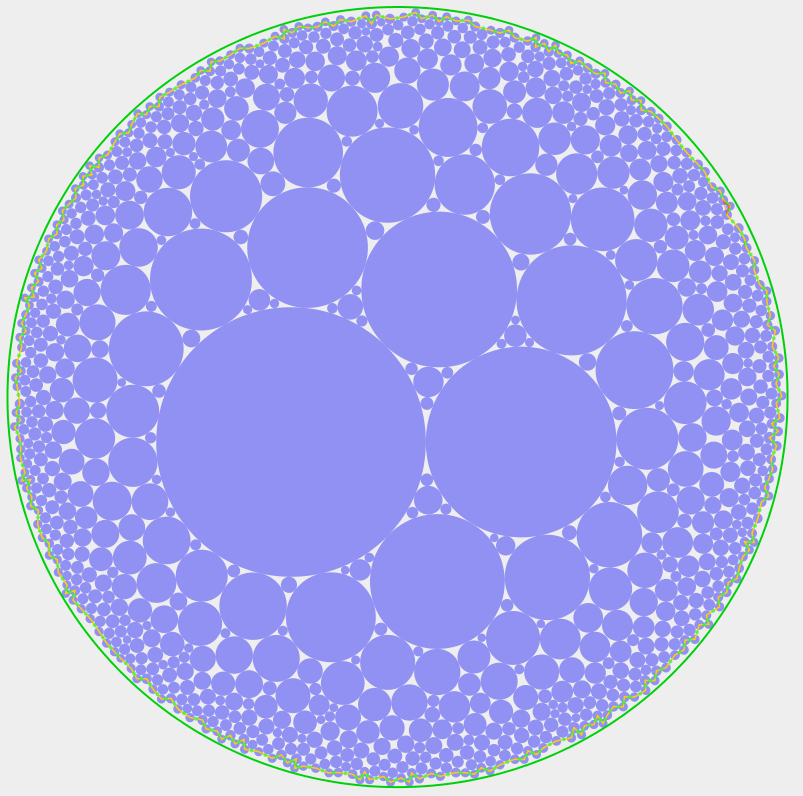
\includegraphics[width=0.65\textwidth]{packing-neg1div2-1000.png}
  \caption{\textit{Packing} voor 1000 cirkels met verdeling $r_i=i^{-1/2}$} \label{fig:packing-neg1div2-1000} 
\end{figure}

\subsubsection{Bespreking}

Deze resultaten zijn volgens mij zeer indrukwekkend.
Resultaten voor de problemen $r_i = i$, $r_i = i^{1/2}$, $r_i = i^{-1/2}$ en $r_i = i^{-2/3}$ blijven steeds onder 10\% vergroting tegenover de best gekende.
Enkel het probleem $r_i = i^{-1/5}$ heeft enkele uitschieters tot maximum 13,45\% vergroting.
Dit laatste resultaat komt waarschijnlijk omdat $r_i = i^{-1/5}$ het probleem is waarin de cirkels het minst verschillen van grootte (zie \autoref{fig:packomania-verdelingen}).
Dit zorgt er voor dat het algoritme minder gebruik kan maken van \textit{holes}, aangezien meestal enkel de kleinere cirkels \textit{holes} zullen opvullen.
Het probleem met het meeste verschil in radii, $r_i = i^{-2/3}$, heeft dan ook de beste resultaten.
Met maximum 4,77\% vergroting en gemiddeld slechts 2,78\%.

Ook is er een duidelijke neerwaartse trend zichtbaar in de vergroting van de omschreven cirkel als het aantal cirkels groter wordt.
Dit komt omdat het algoritme dan meer keuzemogelijkheden heeft in elke stap.
Hierdoor zal het algoritme vaker \textit{holes} kunnen opvullen, en een dichtere \textit{shell} opbouwen.
De kracht van het algoritme is dus het duidelijkst zichtbaar wanneer er genoeg verschillende cirkels zijn om uit te kiezen.

Bovendien worden deze resultaten zeer snel bekomen.
Waar andere algoritmen uit de literatuur uren nodig hebben, vraagt mijn algoritme slechts milliseconden.

Dit zijn denk ik de meest indrukwekkende resultaten van deze thesis, en tonen het best de kracht van het algoritme.

\section{Grotere aantallen cirkels}

Het algoritme uit deze thesis laat ook toe om problemen met veel grotere aantallen cirkels op te lossen.
Resultaten voor 1000 tot 14000 cirkels zijn te vinden in \autoref{append:packomania-tabellen-groter-aantal-cirkels}.
Ik heb geen andere methoden gevonden die problemen met zo'n grote aantallen cirkels kunnen oplossen.
De verkregen radii van de omschreven cirkel kan ik dus niet vergelijken.

De nodige tijd om deze problemen op te lossen blijft ook beperkt.
Problemen tot 1400 cirkels blijven onder één seconde.
Problemen tot 9000 cirkels onder 10 seconden, en 14000 cirkels vragen minder dan één minuut tijd.

Bij deze grote aantallen cirkels komen echter wel enkele problemen naar boven, zoals beschreven in \autoref{chap:bedenkingen}.
Ook was het niet mogelijk op mijn computer om problemen met meer dan 14000 cirkels op te lossen.
Bij het nakijken van de oplossing wordt een recursief algoritme gebruikt op de volledige lijst cirkels.
Dit geeft een \textit{stack-overflow} en heb ik nog niet kunnen oplossen. %CMT - mogelijk pistes voor oplossingen?%

Ondanks de resterende problemen met overlap voor sommige van deze problemen met grote aantallen cirkels, zijn dit interessante resultaten.
Zelfs voor duizenden cirkels kan het algoritme een resultaat geven in enkele seconden.
Dit is, voor zover ik weet, niet mogelijk met andere algoritmen in aanvaardbare tijd, laat staan in enkele seconden.

\section{Conclusie}

In dit hoofdstuk heb ik oplossingen verkregen door mijn algoritme te vergelijken met de best gekende \textit{packings}.
Ook heb ik de nodige rekentijd vergeleken met enkele andere algoritmen.

De oplossingen verkregen met mijn nieuwe constructieve heuristiek hebben een gemiddeld minder dan 6\% grotere omschreven cirkel.
Dit lijkt mij een zeer aanvaardbare vergroting van de omschreven cirkel, rekening houdend met het feit dat het nieuwe algoritme deze problemen in slechts milliseconden op lost.
Zelfs de grootste problemen, bestaande uit duizenden cirkels, kunnen in slechts enkele seconden opgelost worden.
Ook is er een interessante neerwaartse trend in de vergroting van de radius van de bekomen omschreven cirkel.
Dit toont de kracht van het algoritme wanneer het meer cirkels heeft met verschillende radii om uit te kiezen.

Bovendien laat het algoritme toe om problemen met veel grotere aantallen cirkels in aanvaardbare tijd op te lossen.
Voor zover ik weet is er geen enkel ander algoritme dat dit mogelijk maakt voor cirkels met verschillende radii.

\chapter{Verder werk} \label{chap:verder-werk}

In dit hoofdstuk geef ik enkele voorstellen voor verdere uitwerkingen van het algoritme.
Mogelijke verbeteringen, zowel in snelheid als kwaliteit (de grootte van de bekomen omcirkel) van uitkomsten.
Dit zijn mogelijke ideeën om in de toekomst op verder te werken.

\section{Constante-tijd omschreven cirkel}

In het algoritme wordt bij het plaatsen van een cirkel op de \textit{shell} gebruik gemaakt van de omschreven cirkel van de huidige tussen-oplossing.
Deze omschreven cirkel wordt berekend in lineaire tijd ten opzichte van het aantal cirkels op de \textit{shell}.
Dit geeft dan de kleinst mogelijke omschreven cirkel van de huidige oplossing.

Het is echter mogelijk om in constante tijd een omschreven cirkel te berekenen.
Simpelweg door, telkens er een cirkel geplaatst wordt buiten de huidige omschreven cirkel, een nieuwe te berekenen die rond de oude omcirkel en deze nieuwe cirkel past.
Dit kan zeer eenvoudig in constante tijd, maar geeft niet de kleinst-mogelijke omschreven cirkel voor de \textit{packing}.
Deze constante-tijd omschreven cirkel is mogelijk wel goed genoeg als benadering, en kan een grote snelheids-winst geven voor zeer grote \textit{packings}.

\section{Best-Fit}

Het algoritme is gebaseerd op een \textit{best-fit} principe.
Met andere woorden in elke stap wordt de best-passende cirkel gekozen.
Welke cirkel het best past is echter moeilijk te definieren.
In de huidige implementatie worden er daarom enkele keuzes gemaakt, gebaseerd op bestaande heuristieken en eigen intuïtie.
Hier kunnen echter andere keuzes gemaakt worden, die mogelijk tot betere resultaten zullen leiden.

Eén voorbeeld van een alternatieve keuze is bij het plaatsen van een cirkel op de \textit{shell}.
Nu worden de nieuwe cirkels zo dicht mogelijk bij het huidige middelpunt geplaatst.
Dit gebeurt omdat de omschreven cirkel dan zo weinig mogelijk uitgebreid moet worden.
Maar wat als, wanneer we geen cirkel meer binnen de huidige omcirkel kunnen plaatsen, we de cirkel zo ver mogelijk van het middelpunt plaatsen (maar wel nog tegen twee cirkels op de \textit{shell})?
Dit zal er voor zorgen dat de omschreven cirkel veel verder uitgebreid zal worden.
Het zal er ook voor zorgen dat de omcirkel veel minder vaak uitgebreid moet worden, omdat hij in grotere stappen uitbreidt.
Mogelijk geeft dit aanleiding tot betere en misschien snellere \textit{packings} omdat de omschreven cirkel minder vaak herberekend moet worden.

\chapter{Conclusie} \label{chap:conclusie}

In deze thesis heb ik een nieuwe constructieve heuristiek voorgesteld voor het oplossen van het circle-packing probleem.
Deze is gebaseerd op het \textit{best-fit} principe, waarbij in elke stap de beste cirkel gekozen wordt om aan de oplossing toe te voegen.
Deze nieuwe heuristiek gebruikt twee nieuwe concepten: \textit{holes} en de \textit{shell}.
Eerst worden de \textit{holes} opgevuld, daarna worden de cirkels geplaatst aan de buitenkant van de tussen-oplossing, op de \textit{shell}.
Door enkele veronderstellingen te maken over het aantal cirkels die getest moeten worden voor overlap bij elke plaatsing, kan het algoritme zeer snel goede \textit{packings} genereren.
In deze thesis worden de resultaten voor een groot aantal cirkel-verdelingen getoond en vergeleken met gekende \textit{packings} uit de literatuur.
Deze tonen aan dat het algoritme goede \textit{packings} maakt in vergelijking met bestaande algoritmen.
Deze \textit{packings} werden gegenereerd in een fractie van de tijd die andere, \textit{state-of-the-art} algoritmen, nodig hebben (milliseconden tegenover uren).

% // TODO: Extra speculatie over gebruik van mijn algoritme? - ja, dat zette ik ook al in mijn opmerkingen

Daarom denk ik dat ik geslaagd ben in mijn opzet: het maken van een constructief algoritme dat in real-time goede \textit{packings} kan maken voor het \textit{cirkel-packing} probleem.

% // TODO ALGEMEEN: Minder informele termen? Omcirkel->omschreven cirkel < Bwa. Ik dacht dat omcirkel echt een woord was, maar ge hebt dat verzonnen ofwa?

% // TODO ALGEMEEN: Voeg echte definities toe, bv bij Hole echt een hoofding "Definitie" en dan het gat definieren. Ook voor shell, omcirkel.

\newpage

% Bibliography

\bibliography{thesis}
\bibliographystyle{plain}

% Appendixes

\appendix

\chapter{Packomania Benchmark Verdelingen} \label{append:packomania-benchmark-verdelingen}

\begin{tabularx}{\textwidth}{ l c X }
\caption{Packomania Benchmark Verdelingen}
\\\toprule
Instantie & N & Radii \\
\midrule
\endhead
NR10-1 & 10 & 10, 12, 15, 20, 21, 30, 30, 30, 40, 50 \\
NR11-1 & 11 & 8.4, 11, 10, 10.5, 12, 14, 15, 20, 20, 25, 25 \\
NR12-1 & 12 & 11, 12, 13, 14, 15, 16, 17, 18, 19, 20, 21, 22 \\
NR14-1 & 14 & 11, 14, 15, 16, 17, 19, 23, 27, 31, 35, 36, 37, 38, 40 \\
NR15-1 & 15 & 3, 3, 4, 4, 4.5, 6, 7.5, 8, 9, 10, 11, 12, 13, 14, 15 \\
NR15-2 & 15 & 1, 2, 3, 4, 5, 6, 7, 8, 9, 10, 11, 12, 13, 14, 15 \\
NR16-1 & 16 & 13, 14, 15, 15, 17, 19, 23, 26, 27, 27, 32, 37, 38, 47, 57, 63 \\
NR16-2 & 16 & 21, 22, 23, 24, 25, 26, 27, 28, 29, 30, 31, 32, 33, 34, 35, 36 \\
NR17-1 & 17 & 5, 5, 5, 5, 5, 5, 5, 5, 5, 5, 10, 10, 10, 15, 15, 20, 25 \\
NR18-1 & 18 & 12, 14, 16, 23, 25, 26, 27, 28, 33, 35, 47, 49, 53, 53, 55, 60, 67, 71 \\
NR20-1 & 20 & 4, 6, 8, 10, 12, 14, 16, 18, 20, 22, 24, 26, 28, 30, 32, 34, 36, 38, 40, 42 \\
NR20-2 & 20 & 6, 8, 9, 12, 12, 15, 16, 18, 20, 21, 24, 24, 27, 28, 30, 32, 33, 36, 40, 44 \\
NR21-1 & 21 & 10, 15, 16, 17, 17, 18, 21, 22, 23, 25, 26, 31, 33, 34, 37, 37, 38, 39, 40, 42, 45 \\
NR23-1 & 23 & 14, 14, 16, 18, 18, 21, 22, 23, 26, 28, 28, 32, 34, 34, 36, 37, 39, 41, 45, 48, 49, 49, 51 \\
NR24-1 & 24 & 9, 10, 11, 13, 13, 16, 17, 17, 18, 19, 19, 20, 20, 20, 21, 22, 23, 23, 24, 25, 30, 31, 32, 82 \\
NR25-1 & 25 & 14, 17, 22, 26, 26, 27, 28, 29, 29, 30, 31, 32, 33, 34, 34, 34, 34, 35, 37, 37, 37, 47, 52, 53, 55 \\
NR26-1 & 26 & 31, 32, 33, 34, 35, 36, 37, 38, 39, 40, 41, 42, 43, 44, 45, 46, 47,48, 49, 50, 51, 52, 53, 54, 55, 56 \\
NR26-2 & 26 & 41, 42, 43, 44, 45, 46, 47, 48, 49, 50, 51, 52, 53, 54, 55, 56, 57,58, 59, 60, 61, 62, 63, 64,65, 66 \\
NR27-1 & 27 & 17, 21, 25, 26, 26, 27, 27, 28, 29, 33, 33, 34, 35, 35, 35, 37, 40, 42, 43, 44, 45, 49, 53, 55, 55, 55, 63 \\
NR30-1 & 30 & 5, 8, 10, 10, 12, 14, 15, 16, 18, 20, 20, 20, 20, 20, 22, 24, 25, 26, 30, 30, 30, 30, 35, 40,40, 45, 48, 50, 55, 60 \\
NR30-2 & 30 & 6, 8, 8, 10, 12, 13, 14, 16, 18, 18, 20, 22, 23, 24, 25, 27, 28, 29,31, 33, 33, 35, 37, 38, 39,41, 43, 43, 48, 53 \\
NR40-1 & 40 & 31, 32, 33, 34, 35, 36, 37, 38, 39, 40, 41, 42, 43, 44, 45, 46, 47,48, 49, 50, 51, 52, 53, 54,55, 56, 57, 58, 59, 60, 61, 62, 63, 64, 65, 66, 67, 68, 69, 70 \\
NR50-1 & 50 & 18, 18, 19, 19, 19, 19, 21, 21, 24, 25, 25, 30, 31, 31, 33, 33, 36,36, 40, 42, 43, 46, 46, 47,49, 49, 49, 50, 50, 54, 56, 56, 57, 57, 58, 58, 59, 59, 59, 61, 62,63, 63, 64, 65, 68, 78, 79,80, 86 \\
NR60-1 & 60 & 35, 35, 35, 36, 37, 37, 38, 38, 39, 39, 40, 41, 41 ,42, 42, 42, 42,42, 44, 44, 45, 45, 46,46,47, 48, 48, 49, 50, 50, 54, 54, 57, 57, 59, 60,60, 71, 71, 71,72, 72, 74, 74, 76, 77, 77,79, 79, 80, 82, 82, 85, 86, 89, 90, 94, 95, 96, 100 \\

IN9-1 & 9 & 10, 10, 10, 10, 4.1415, 4.1415, 4.1415, 4.1415, 4.1415 \\
IN10-1 & 10 & 50, 40, 32, 31.5, 20, 20, 20, 11, 10, 10 \\
IN10-2 & 10 & 50, 40, 30, 30, 30, 21, 20, 15, 12, 10 \\
IN11-1 & 11 & 20, 19, 18, 17, 16, 15, 14, 13, 12, 11, 10 \\
IN11-2 & 11 & 25, 25, 20, 20, 15, 14, 12, 11, 10.5, 10, 8.4 \\
IN12-1 & 12 & 100, 100, 100, 48.26, 48.26, 48.26, 23.72, 23.72, 23.72, 23.72, 23.72, 23.72 \\
IN14-1 & 14 & 40, 38, 37, 36, 35, 31, 27, 23, 19, 17, 16, 15, 14, 11 \\
IN15-1 & 15 & 15, 14, 13, 12, 11, 10, 9, 8, 7, 6, 5, 4, 3, 2, 1 \\
IN16-1 & 16 & 36, 35, 34, 33, 32, 31, 30, 29, 28, 27, 26, 25, 24, 23 ,22, 21 \\
IN17-1 & 17 & 25, 20, 15, 15, 10, 10, 10, 5, 5, 5, 5, 5, 5, 5, 5, 5, 5 \\
IN17-2 & 17 & 100, 100, 100, 100, 41.415, 41.415, 41.415, 41.415, 41.415, 20, 20, 20, 20, 20, 20, 20, 20 \\
IN25-1 & 25 & 10, 10, 10, 3.533, 3.533, 3.533, 3.533, 3.533, 3.533, 2.3, 2.3, 2.3, 1.8, 1.8, 1.8, 1.8, 1.8, 1.8, 1.547, 1.08, 1.08, 1.08, 1.08, 1.08, 1.08 \\
IN28-1 & 28 & 10, 10, 10, 4.826, 4.826, 4.826, 2.371, 2.371, 2.371, 2.371, 2.371, 2.371, 1.547, 1.345, 1.345, 1.345, 1.345, 1.345, 1.345, 1.161, 1.161, 1.161, 0.9, 0.9, 0.9, 0.9, 0.9, 0.9  \\
IN162-1 & 162 & 1.8, 1.8, 1.8, 1.75, 1.3, 1.3, 1.3, 1.3, 1.3, 1.3, 1.3, 1.3, 1.3, 1.3, 1.3, 1.3, 1.05, 1.05, 1.05, 1.05, 1.05, 1.05, 1.05, 1.05, 1.05, 0.9, 0.9, 0.9, 0.9, 0.9, 0.9, 0.9, 0.9, 0.9, 0.9, 0.9, 0.9, 0.9, 0.9, 0.9, 0.8, 0.8, 0.8, 0.8, 0.8, 0.8, 0.8, 0.8, 0.8, 0.8, 0.8, 0.8, 0.8, 0.8, 0.8, 0.8, 0.8, 0.8, 0.8, 0.8, 0.8, 0.8, 0.8, 0.8, 0.8, 0.8, 0.8, 0.8, 0.8, 0.8, 0.8, 0.75, 0.7, 0.7, 0.7, 0.7, 0.7, 0.7, 0.7, 0.7, 0.7, 0.7, 0.7, 0.65, 0.65, 0.65, 0.65, 0.65, 0.65, 0.65, 0.65, 0.65, 0.65, 0.65, 0.65, 0.65, 0.65, 0.65, 0.65, 0.65, 0.65, 0.65, 0.65, 0.65, 0.65, 0.65, 0.65, 0.65, 0.65, 0.65, 0.65, 0.65, 0.65, 0.65, 0.65, 0.65, 0.65, 0.65, 0.65, 0.65, 0.65, 0.65, 0.65, 0.65, 0.65, 0.65, 0.65, 0.65, 0.65, 0.65, 0.65, 0.65, 0.65, 0.65, 0.65, 0.65, 0.65, 0.55, 0.55, 0.55, 0.55, 0.55, 0.55, 0.55, 0.55, 0.55, 0.55, 0.55, 0.55, 0.55, 0.55, 0.55, 0.55, 0.55, 0.55, 0.55, 0.55, 0.55, 0.55, 0.55, 0.55, 0.55 \\
\bottomrule
\end{tabularx}

\chapter{Packomania Vergelijking Tabellen} \label{append:packomania-tabellen}

In deze tabellen wordt telkens het aantal cirkels in de kolom $N$ gegeven, de best gekende radius van op Packomania in kolom $Beste radius$ en de radius verkregen door mijn algoritme in kolom $Radius$.
Ook wordt het absolute verschil van mijn oplossing ten opzichte van de best gekende radius in de kolom $Vergroting$ gegeven, en de procentuele vergroting in kolom $Vergroting (\%)$.
Als laatste wordt de rekentijd die mijn algoritme nodig had om tot deze oplossing te komen gegeven in kolom $Tijd$.

\section{Cirkels met gelijke grootte} \label{append:packomania-tabellen-gelijke-grootte}

Merk op dat voor het \textit{circle-packing} probleem met even grote cirkels enkel de oplossingen voor $N=3$ tot $N=100$ hier getoond worden.
Dit is slechts een subset van alle gekende oplossingen.
De volledige lijst van vergelijkingen voor dit probleem, meer dan 2500 vergelijkingen, kan u terug vinden op GitHub \cite{packomania-tables-github}.

\equalTable{Packomania \ensuremath{r_i=1}}{0}{98} \label{table:packomania-equal}

\section{Packomania Macht problemen} \label{append:packomania-tabellen-macht}

\powerTable{Packomania \ensuremath{r_i=i}}{0}{196} \label{table:packomania-i}

\powerTable{Packomania \ensuremath{r_i=i^{1/2}}}{196}{292} \label{table:packomania-i^1/2}

\powerTable{Packomania \ensuremath{r_i=i^{-1/5}}}{444}{504} \label{table:packomania-i^-1/5}

\powerTable{Packomania \ensuremath{r_i=i^{-1/2}}}{292}{388} \label{table:packomania-i^-1/2}

\powerTable{Packomania \ensuremath{r_i=i^{-2/3}}}{388}{444} \label{table:packomania-i^-2/3}

Opmerking: Een oplossing voor 56 cirkels, met raddii $r_i=i^{-2/3}$ miste op de Packomania website op het moment van het schrijven van deze thesis.

\section{Packomania Benchmark problemen} \label{append:packomania-tabellen-benchmark}

\benchmarkTable{Packomania Benchmark Instances}{0}{1000}

\section{Grotere aantallen cirkels} \label{append:packomania-tabellen-groter-aantal-cirkels}

Enkel de resultaten voor meer dan 1000 cirkels worden hier getoond.
De volledige lijst van grotere problemen, van 100 cirkels tot 14000 cirkels, kan je terug vinden op GitHub \cite{packomania-tables-github}.

\bigTable{Grotere aantallen gelijke cirkels}{130}{153}

\bigTable{Grotere aantallen cirkels: \ensuremath{r_i = i^{1/2}}}{283}{306}

\bigTable{Grotere aantallen cirkels: \ensuremath{r_i = i^{-1/2}}}{436}{459}

\bigTable{Grotere aantallen cirkels: \ensuremath{r_i = i^{-2/3}}}{589}{612}

\bigTable{Grotere aantallen cirkels: \ensuremath{r_i = i^{-1/5}}}{742}{765}

\chapter{Extra \textit{packing} figuren} \label{append:extra-packing-figuren}

% gelijke grootte

\begin{figure}
  \centering
  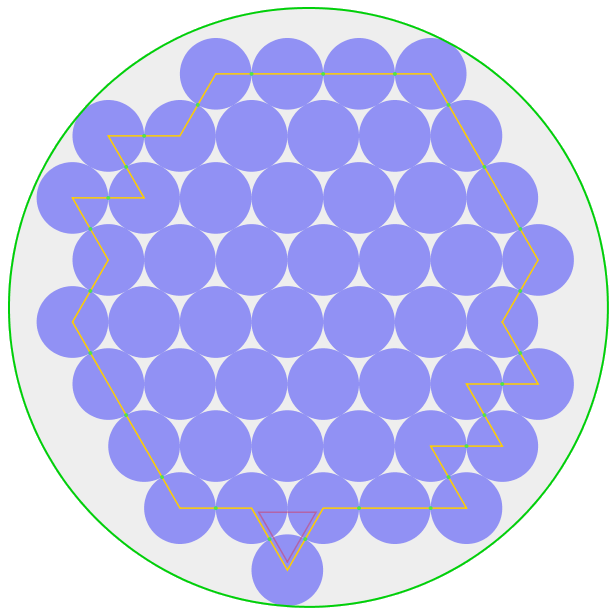
\includegraphics[width=0.65\textwidth]{packing-even-groot-50.png}
  \caption{\textit{Packing} voor 50 cirkels met gelijke grootte}
\end{figure}

\begin{figure}
  \centering
  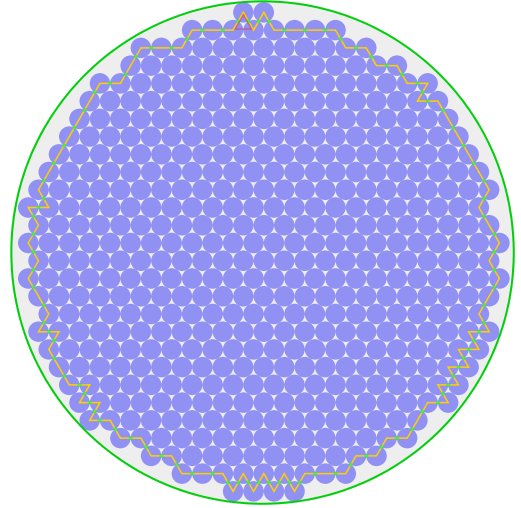
\includegraphics[width=0.65\textwidth]{packing-even-groot-500.png}
  \caption{\textit{Packing} voor 500 cirkels met gelijke grootte}
\end{figure}

\begin{figure}
  \centering
  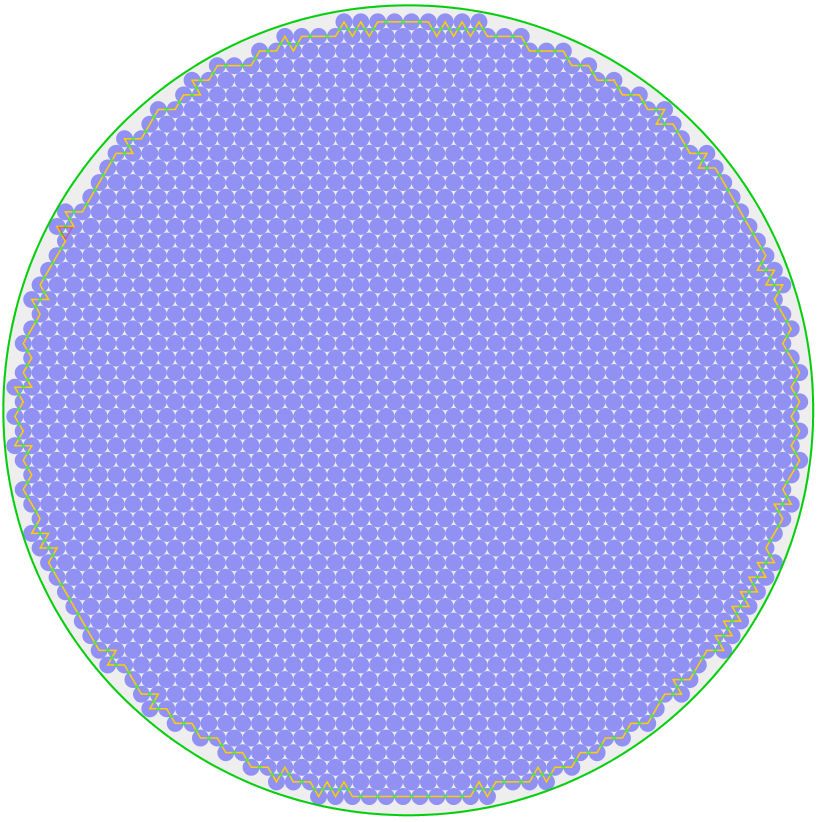
\includegraphics[width=0.65\textwidth]{packing-even-groot-2000.png}
  \caption{\textit{Packing} voor 2000 cirkels met gelijke grootte}
\end{figure}

\begin{figure}
  \centering
  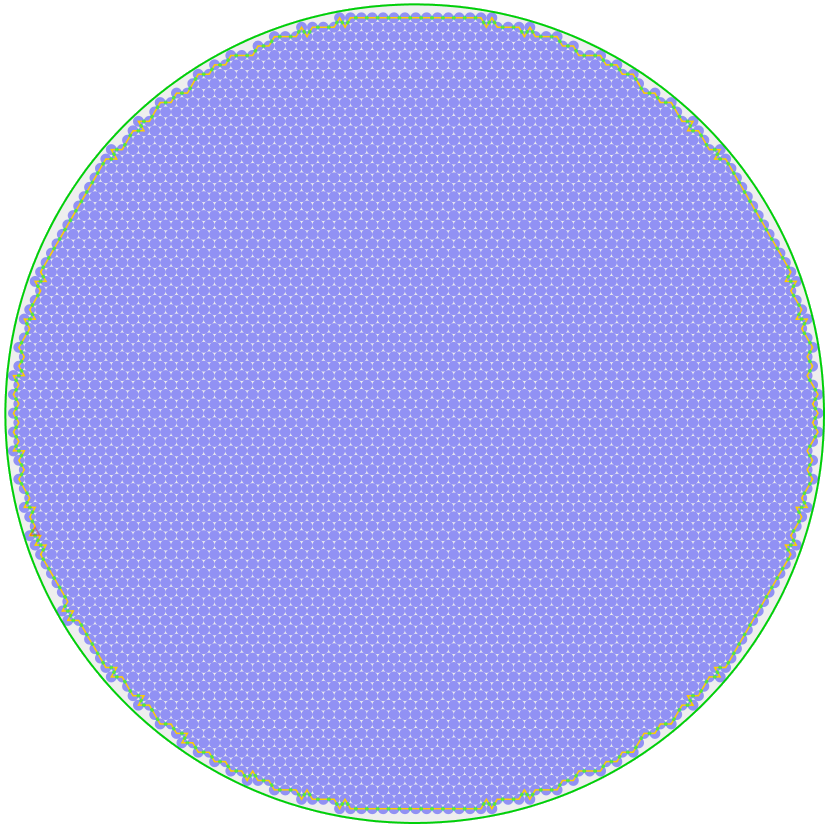
\includegraphics[width=0.65\textwidth]{packing-even-groot-5000.png}
  \caption{\textit{Packing} voor 5000 cirkels met gelijke grootte}
\end{figure}

% Machten

% 100
\begin{figure}
  \centering
  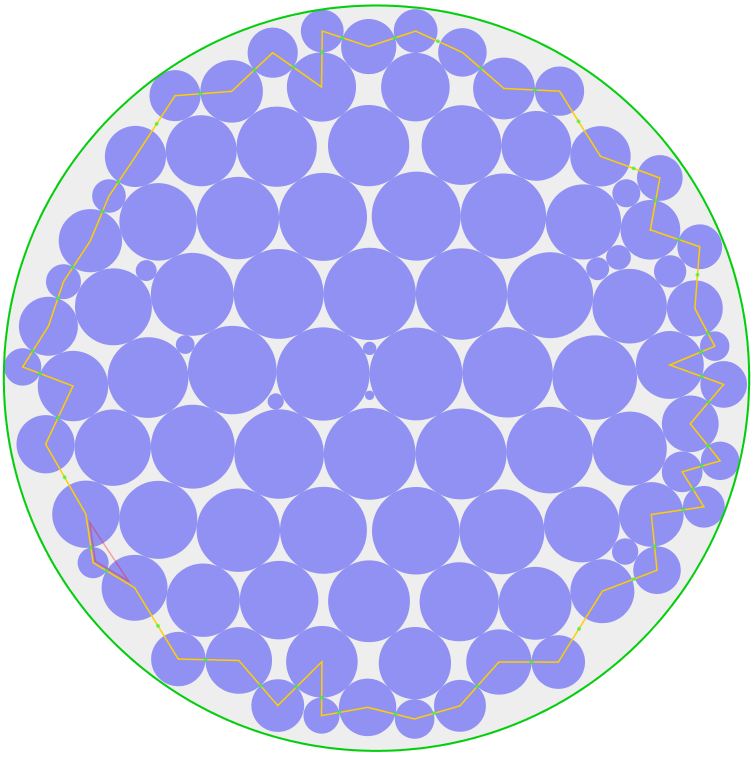
\includegraphics[width=0.65\textwidth]{packing-1div2-100.png}
  \caption{\textit{Packing} voor 100 cirkels met verdeling $r_i=i^{1/2}$}
\end{figure}

\begin{figure}
  \centering
  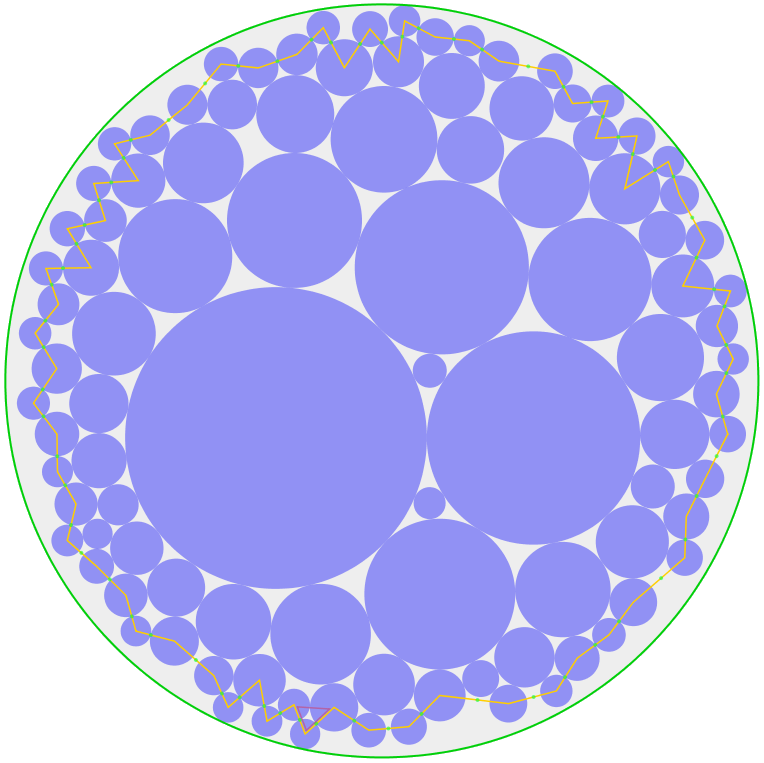
\includegraphics[width=0.65\textwidth]{packing-neg1div2-100.png}
  \caption{\textit{Packing} voor 100 cirkels met verdeling $r_i=i^{-1/2}$}
\end{figure}

\begin{figure}
  \centering
  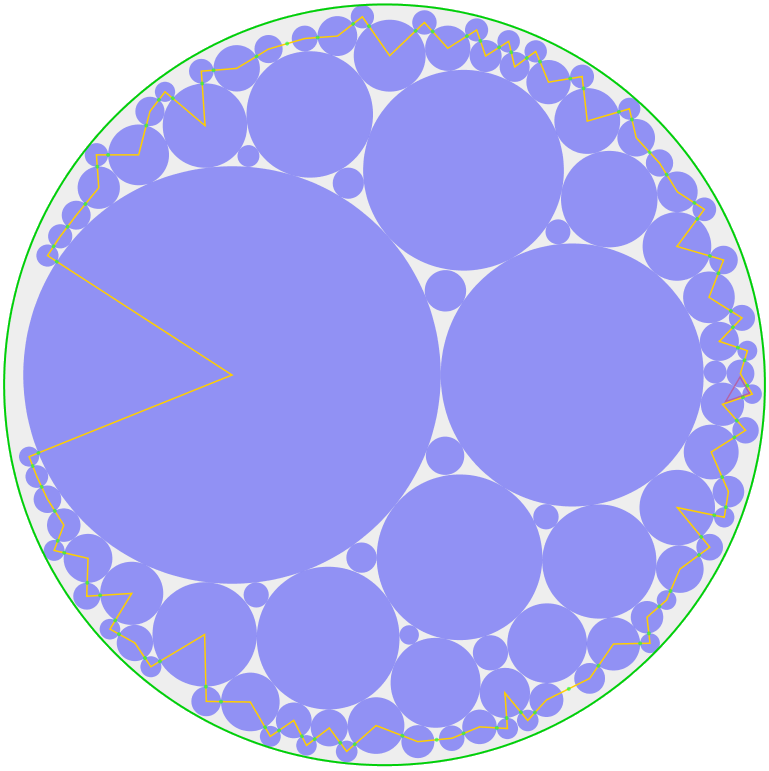
\includegraphics[width=0.65\textwidth]{packing-neg2div3-100.png}
  \caption{\textit{Packing} voor 100 cirkels met verdeling $r_i=i^{-2/3}$}
\end{figure}

\begin{figure}
  \centering
  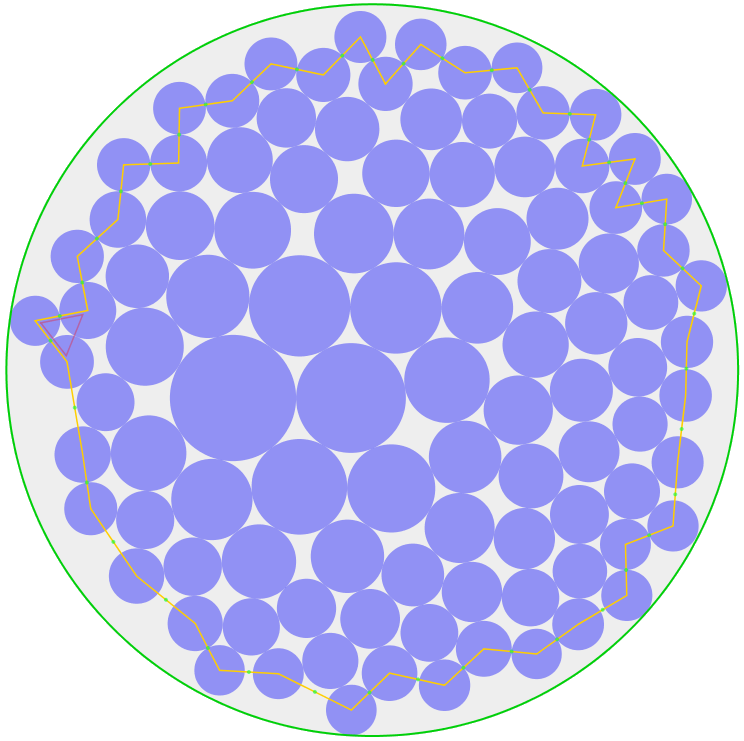
\includegraphics[width=0.65\textwidth]{packing-neg1div5-100.png}
  \caption{\textit{Packing} voor 100 cirkels met verdeling $r_i=i^{-1/5}$}
\end{figure}

% 1000
\begin{figure}
  \centering
  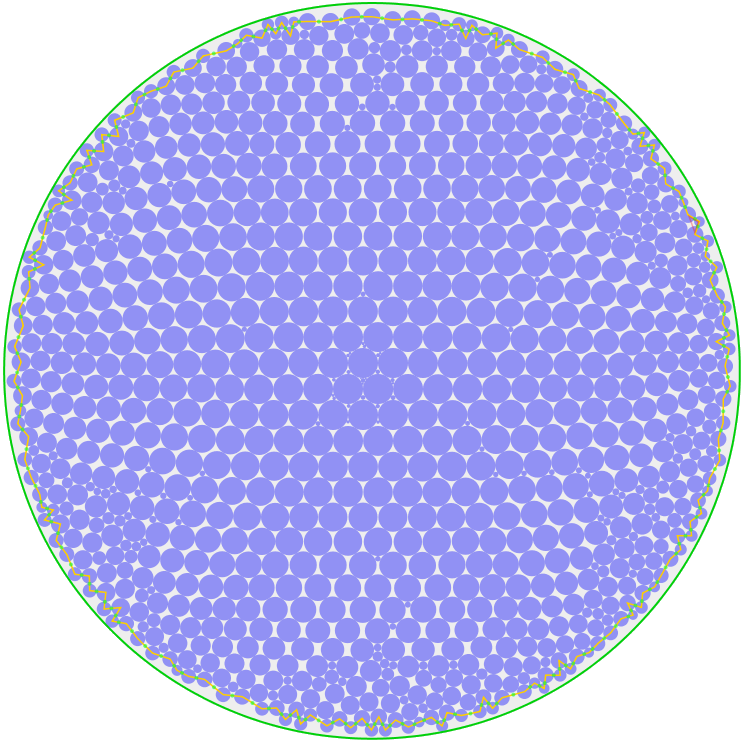
\includegraphics[width=0.65\textwidth]{packing-1div2-1000.png}
  \caption{\textit{Packing} voor 1000 cirkels met verdeling $r_i=i^{1/2}$}
\end{figure}

\begin{figure}
  \centering
  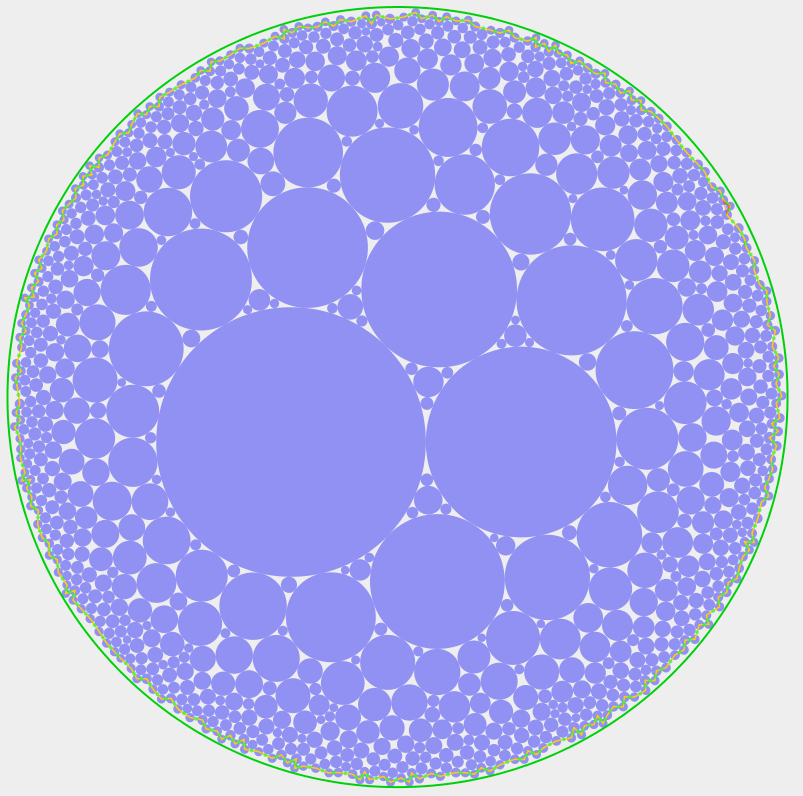
\includegraphics[width=0.65\textwidth]{packing-neg1div2-1000.png}
  \caption{\textit{Packing} voor 1000 cirkels met verdeling $r_i=i^{-1/2}$}
\end{figure}

\begin{figure}
  \centering
  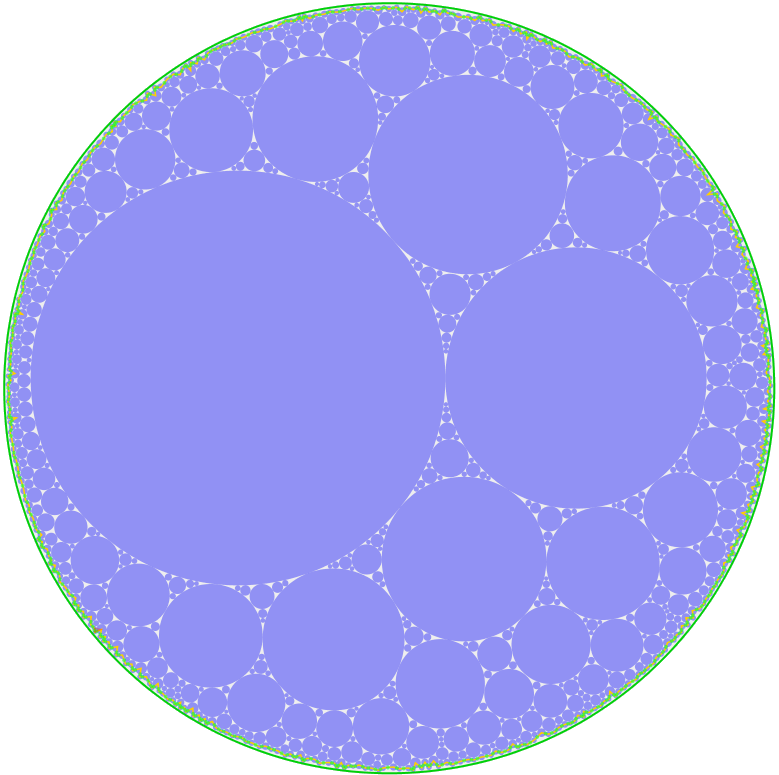
\includegraphics[width=0.65\textwidth]{packing-neg2div3-1000.png}
  \caption{\textit{Packing} voor 1000 cirkels met verdeling $r_i=i^{-2/3}$}
\end{figure}

\begin{figure}
  \centering
  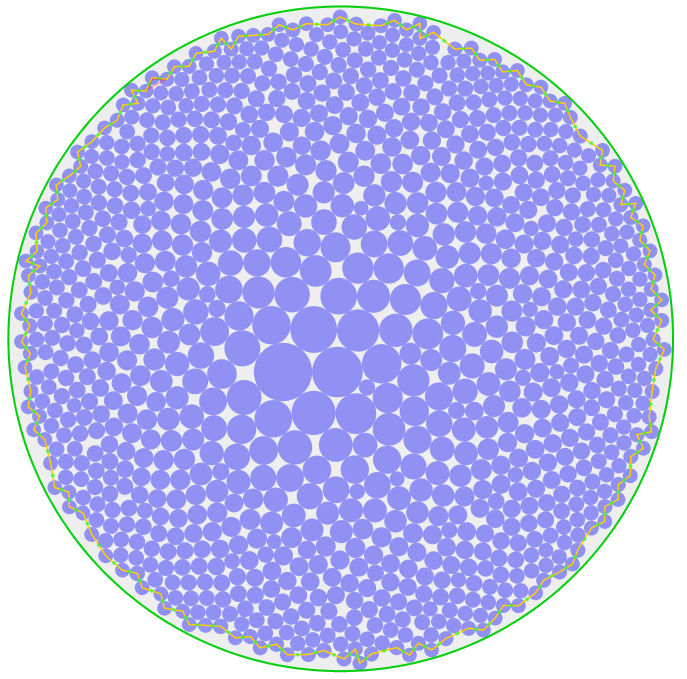
\includegraphics[width=0.65\textwidth]{packing-neg1div5-1000.png}
  \caption{\textit{Packing} voor 1000 cirkels met verdeling $r_i=i^{-1/5}$}
\end{figure}

%5000
\begin{figure}
  \centering
  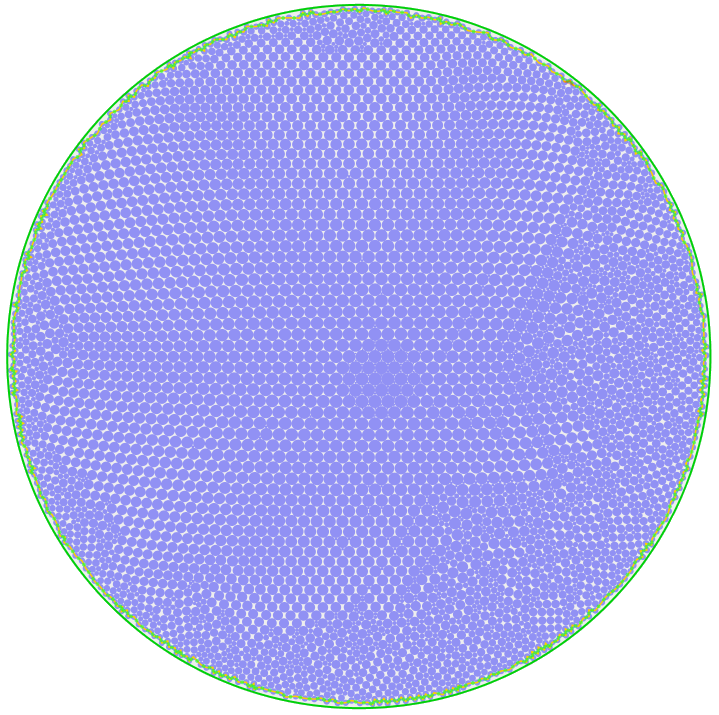
\includegraphics[width=0.65\textwidth]{packing-1div2-5000.png}
  \caption{\textit{Packing} voor 5000 cirkels met verdeling $r_i=i^{1/2}$}
\end{figure}

\begin{figure}
  \centering
  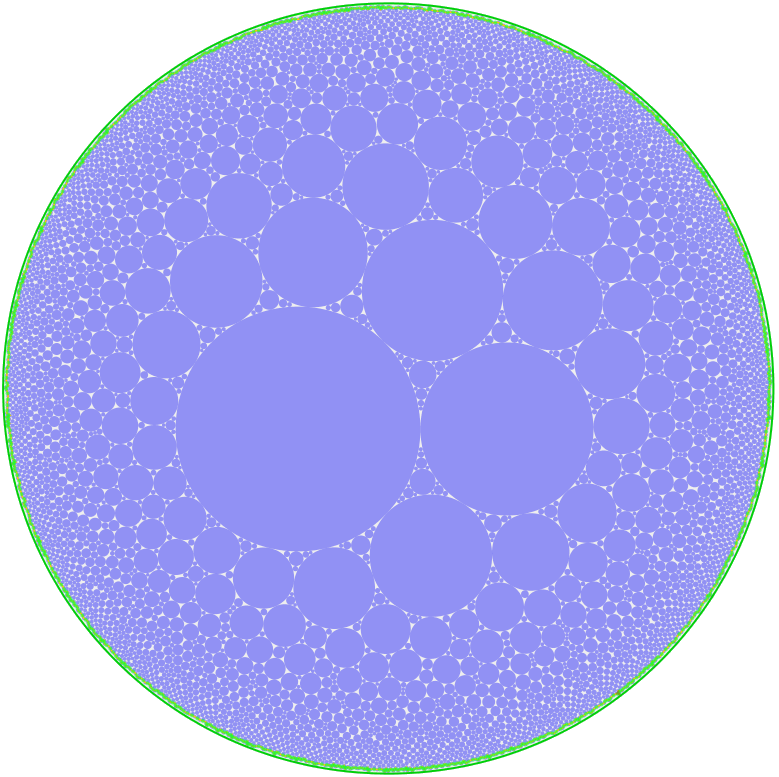
\includegraphics[width=0.65\textwidth]{packing-neg1div2-5000.png}
  \caption{\textit{Packing} voor 5000 cirkels met verdeling $r_i=i^{-1/2}$}
\end{figure}

\begin{figure}
  \centering
  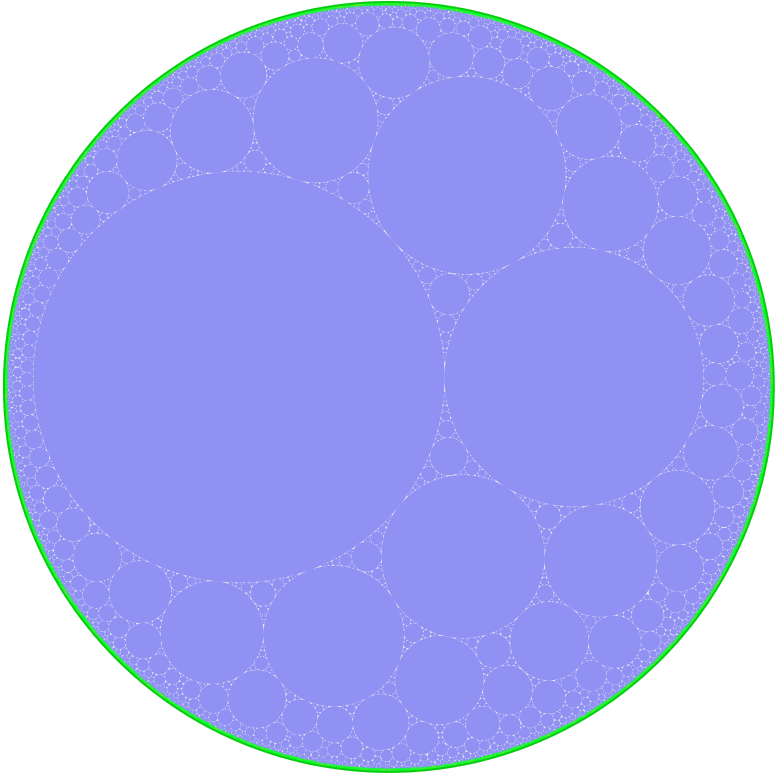
\includegraphics[width=0.65\textwidth]{packing-neg2div3-5000.png}
  \caption{\textit{Packing} voor 5000 cirkels met verdeling $r_i=i^{-2/3}$}
\end{figure}

\begin{figure}
  \centering
  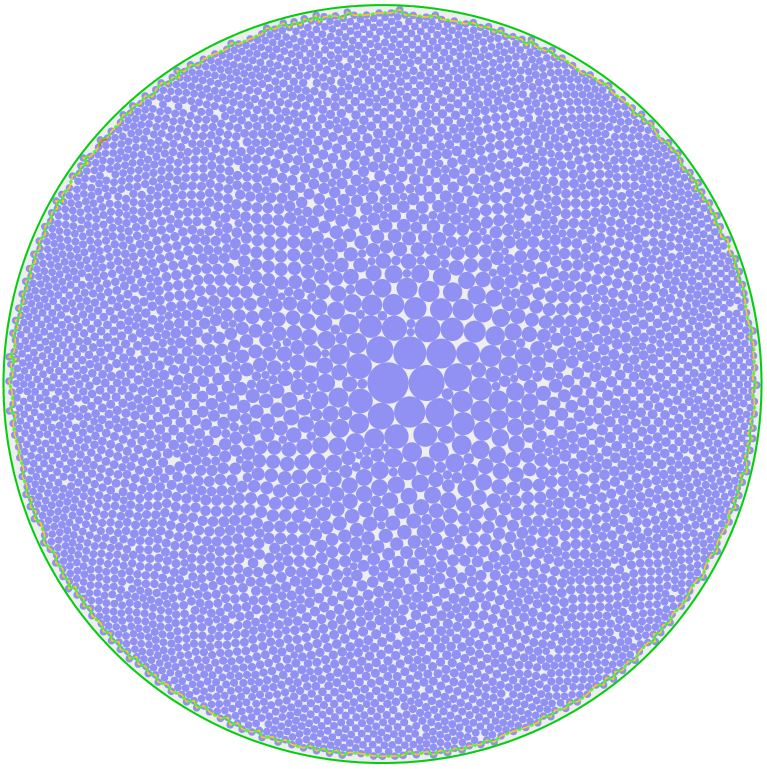
\includegraphics[width=0.65\textwidth]{packing-neg1div5-5000.png}
  \caption{\textit{Packing} voor 5000 cirkels met verdeling $r_i=i^{-1/5}$}
\end{figure}

\newpage

% ----------------------- Achterblad ------------------------------
% Vergeet niet de tekst aan te passen:
% - Afdeling
% - Adres van de afdeling
% - Telefoon en faxnummer
% -----------------------------------------------------------------
\thispagestyle{empty}
\sffamily
%
\begin{textblock}{191}(113,-11)
{\color{blueline}\rule{160pt}{5.5pt}}
\end{textblock}
%
\begin{textblock}{191}(168,-11)
{\color{blueline}\rule{5.5pt}{59pt}}
\end{textblock}
%
\begin{textblock}{183}(-24,-11)
\textblockcolour{}
\flushright
\fontsize{7}{7.5}\selectfont
\textbf{COMPUTERWETENSCHAPPEN}\\
Celestijnenlaan 200A - bus 2402\\
3001 HEVERLEE, BELGI\"{E}\\
tel. + 32 16 32 77 00\\
fax + 32 16 32 79 96\\
www.kuleuven.be\\
\end{textblock}
%
\begin{textblock}{191}(154,-7)
\textblockcolour{}
\includegraphics*[height=16.5truemm]{sedes.png}
\end{textblock}
%
\begin{textblock}{191}(-20,235)
{\color{bluetitle}\rule{544pt}{55pt}}
\end{textblock}
\end{document}
